\section{Results}

\Cref{fig:dem_ts_aug_04_2011}, \cref{fig:dem_ts_aug_31_2012} and \cref{fig:dem_ts_oct_28_2021} shows the timeseries plot of DEM for the three events. The time series plot is calculated by averaging the acceptable DEM solutions obtained for each image over three consecutive temperature range (i.e averaging the solutions for 5.85, 5.9 and 5.95 etc.). Blue curve corresponds to the full disk DEM and red curve corresponds to the point source DEM. The temperature range above logT=6.75 has been omitted as no correlation was found between point source and full disk.

\begin{figure}[h!]
    \centering
    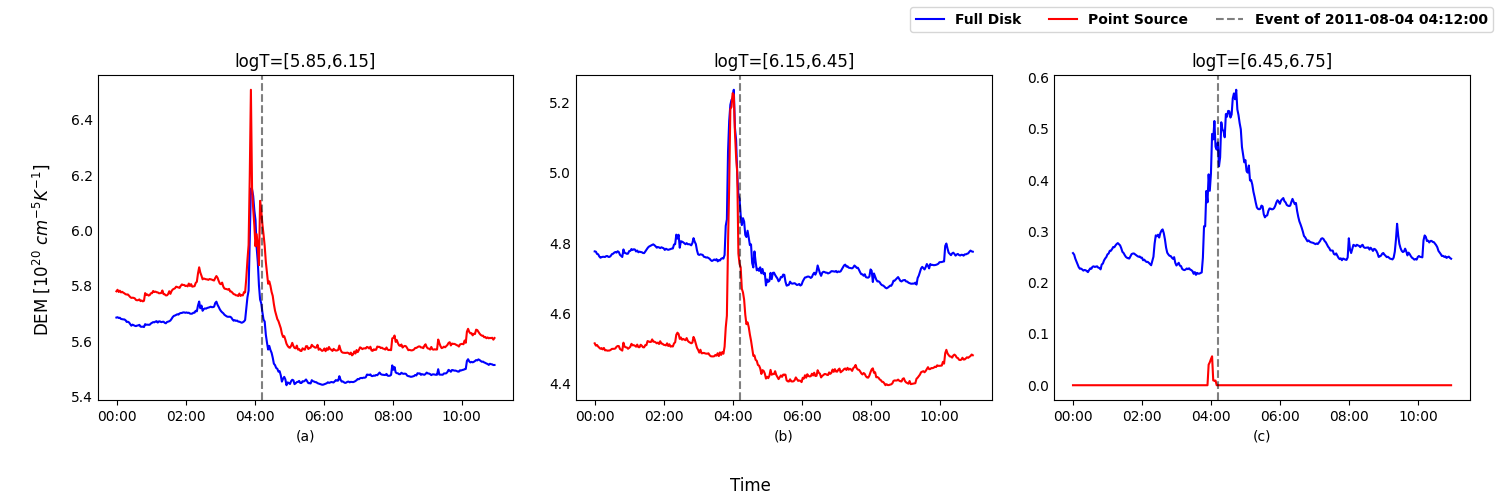
\includegraphics[width=\textwidth]{images/dem_ts_aug_04_2011.png}
    \caption[DEM Timeseries for August 2011 Event]{Timeseries of DEM for \nth{4} August 2011 Event.}
    \label{fig:dem_ts_aug_04_2011}
\end{figure}

\begin{figure}[h!]
    \centering
    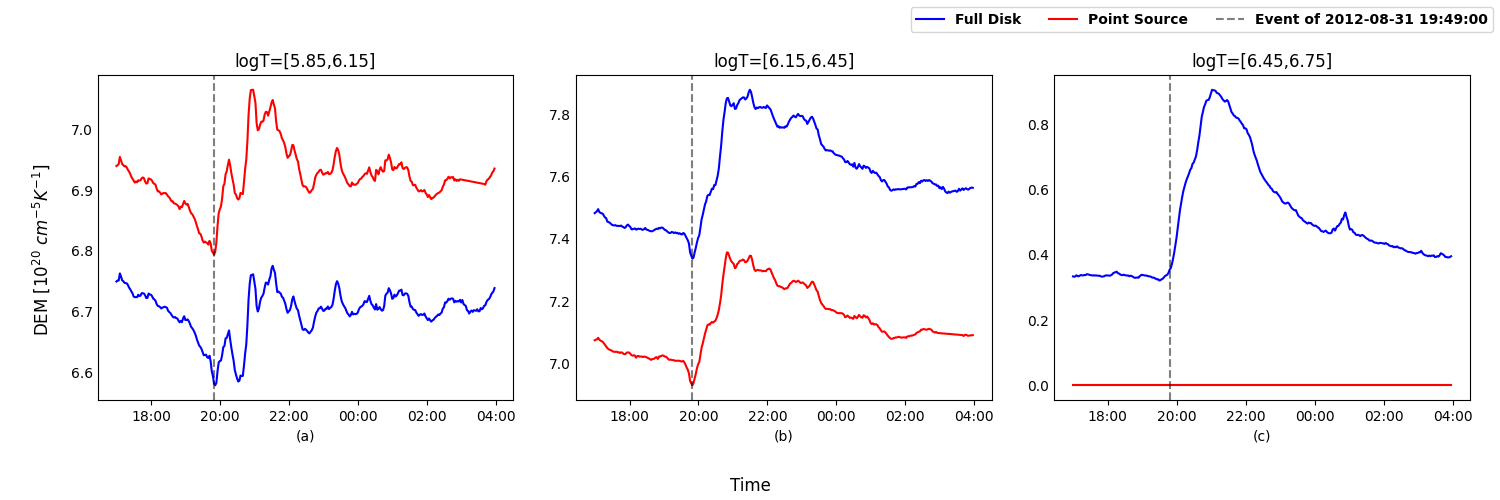
\includegraphics[width=\textwidth]{images/dem_ts_aug_31_2012.png}
    \caption[DEM Timeseries for August 2012 Event]{Timeseries of DEM for \nth{31} August 2012 Event}
    \label{fig:dem_ts_aug_31_2012}
\end{figure}

\begin{figure}[h!]
    \centering
    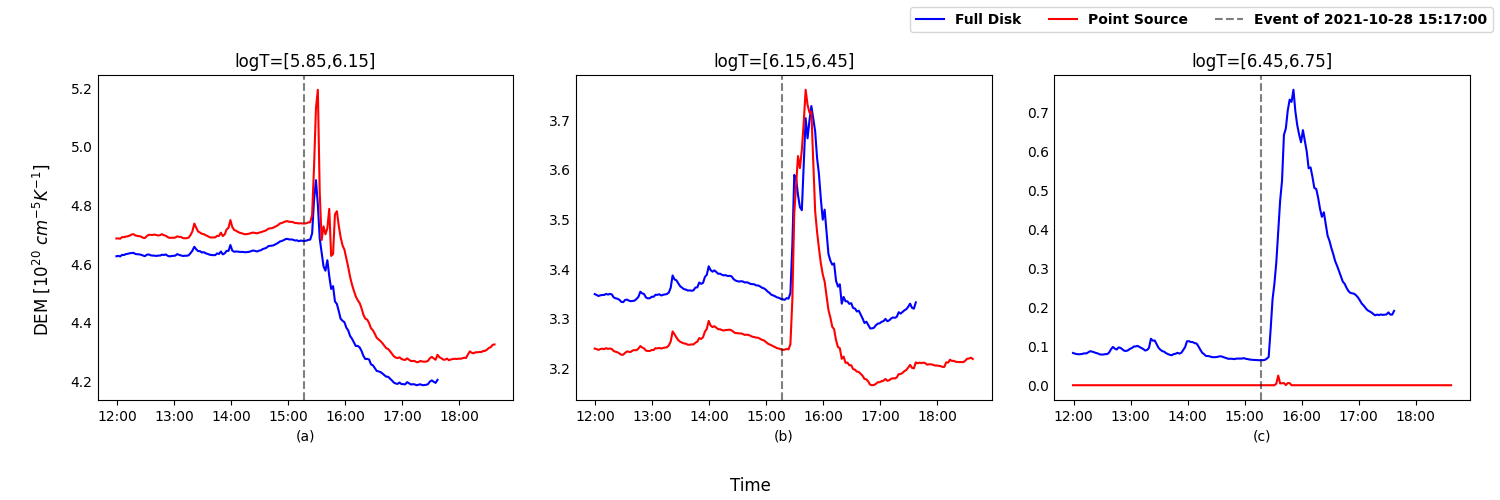
\includegraphics[width=\textwidth]{images/dem_ts_oct_28_2021.png}
    \caption[DEM Timeseries for October 2021 Event]{Timeseries of DEM for \nth{28} October 2021 Event}
    \label{fig:dem_ts_oct_28_2021}
\end{figure}

In \cref{fig:dem_ts_aug_04_2011}(a) and \cref{fig:dem_ts_aug_04_2011}(b), we can observe the coronal dimming or decrease in the DEM value after the event spike. But, in \cref{fig:dem_ts_aug_04_2011}(c) no dimming is observed. Dimming is the most prominent in logT = [5.85, 6.15]. The sudden increase in the DEM curve is due to the solar flare which is associated with the CME. There is very high correlation for the first two temperature ranges, but there is little to no correlation in the DEM profiles of the full disk and point source for the temperature range logT=[6.45, 6.75]. For temperature ranges greater than logT=6.45, the correlation is almost 0. We make use of Pearson's Correlation coeffecient (\cref{eqn:pearsonr}) to find out the amount of correlation between the point source and full disk DEM, for which we use \texttt{pearsonr} function from the \texttt{scipy} library in Python. The pearson correlation coeffecient r between two datasets \textbf{x} and \textbf{y} is calculated using the formula,

\begin{equation}
    \label{eqn:pearsonr}
    r = \frac{\sum (x_i - \overline{x})(y_i - \overline{y})}{\sqrt{\sum (x_i - \overline{x})^2 \sum (y_i - \overline{y})^2}}
\end{equation}\hspace{0.25cm}

\begin{table}[h!]
    \centering
    \begin{tblr}{
          cell{1}{1} = {r=2}{},
          cell{1}{2} = {c=3}{c},
          vline{1-5} = {-}{},
          hline{1-6} = {-}{},
        }
        \textbf{Event} & \textbf{Pearson Correlation Coeffecient} &         & \\
        & logT=[5.85, 6.15]  & logT=[6.15, 6.45] & logT=[6.45, 6.75] \\
        \nth{4} August 2011  & 0.9449 & 0.9767 & 0.2190\\
        \nth{31} August 2012  & 0.7027 & 0.9885 & 0.2079\\
        \nth{28} October 2021 & 0.9555 & 0.9577 & 0.2578 \\
    \end{tblr}
    \caption{Correlation between Point source and Full Disk DEM}
\end{table}

We see a discrepancy in the value of DEM between the point source and full disk average values. This could be due to the error induced during the DEM profile reconstruction, instrumental errors, error incurred during the resampling or reduction of image dimension from 4096 $\times$ 4096 pixels to 512 $\times$ 512 and it could also be due to averaging error. The dataset length is not equal in some of the case as invalid or small DEM solution values have been removed.\\

The temperature distribution of the plasma at different sections of an event can be studied through it's DEM profile (DEM profile is a plot of logT vs DEM). The DEM profiles before, during and after the event has been shown in \cref{fig:dem_pro_aug_04_2011}, \cref{fig:dem_pro_aug_31_2012} and \cref{fig:dem_pro_oct_28_2021} for the events of \nth{4} August 2011, \nth{31} August 2012 and \nth{28} October 2021 respectively.

\begin{figure}[h!]

    \begin{subfigure}[b]{0.3\textwidth}
        \centering
        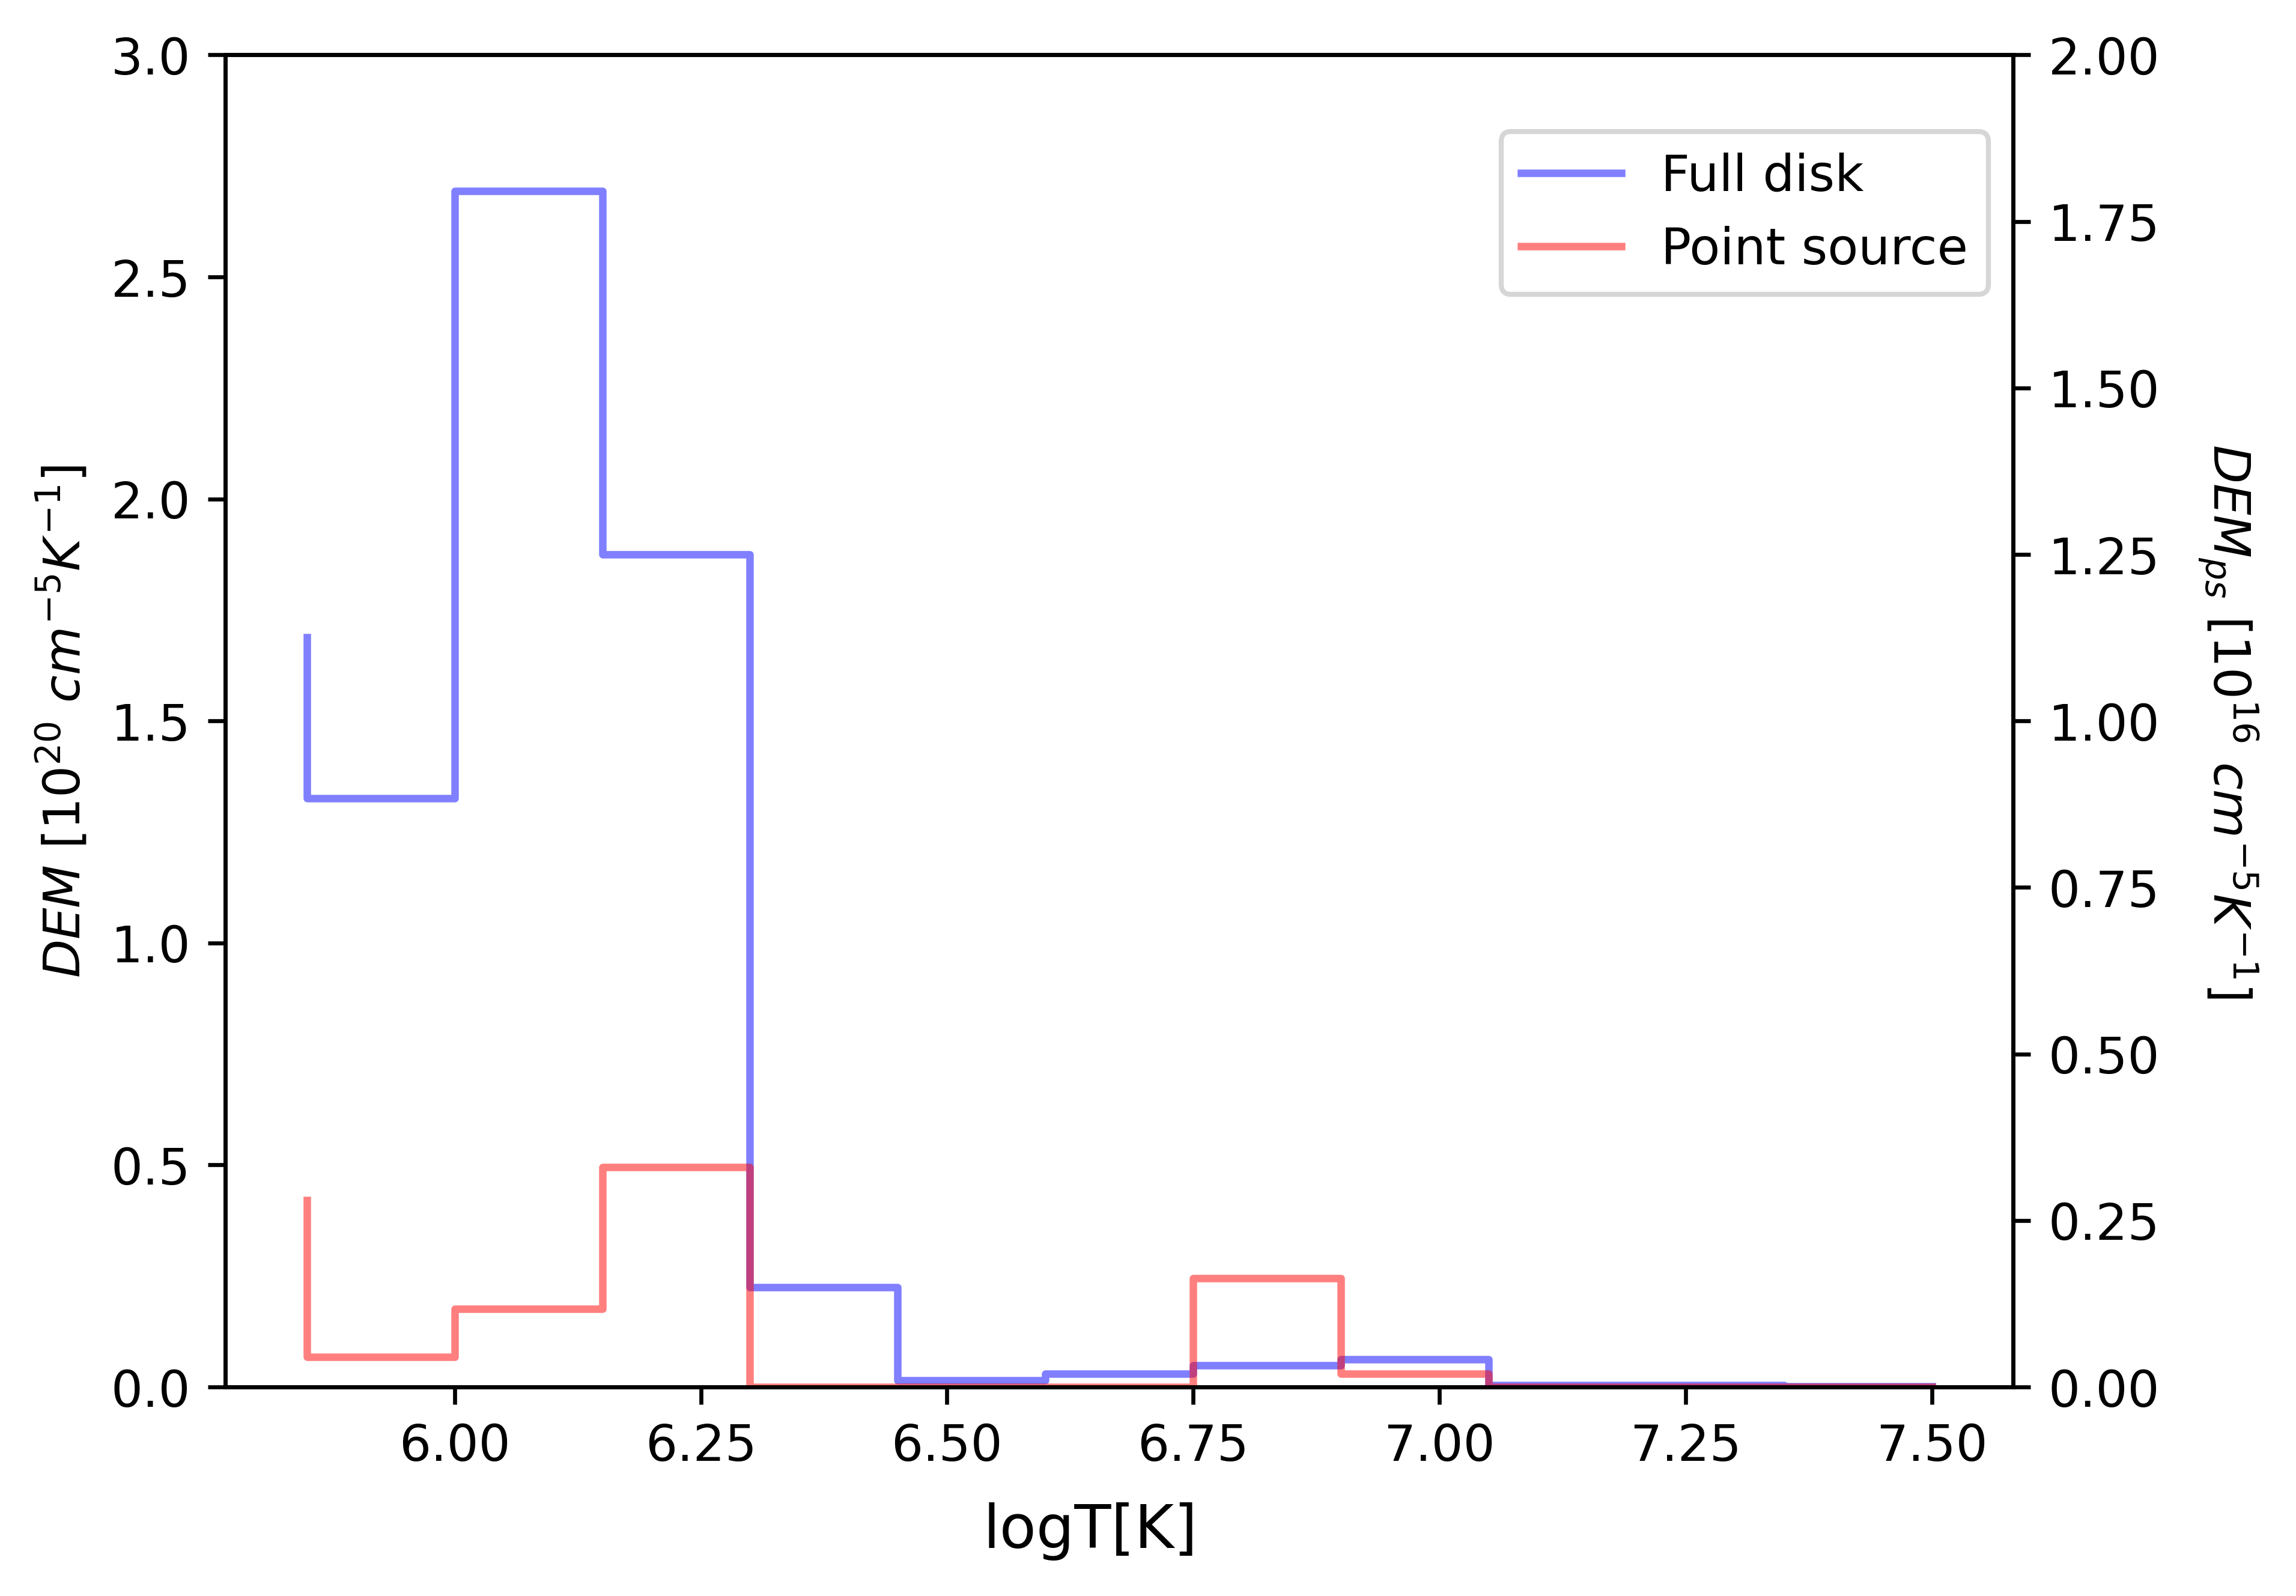
\includegraphics[width=\textwidth]{images/dem_profile_before_event_2011_aug_04.png}
        \caption{Before event (02:21 UT)}
    \end{subfigure}
    \hfill
    \begin{subfigure}[b]{0.3\textwidth}
        \centering
        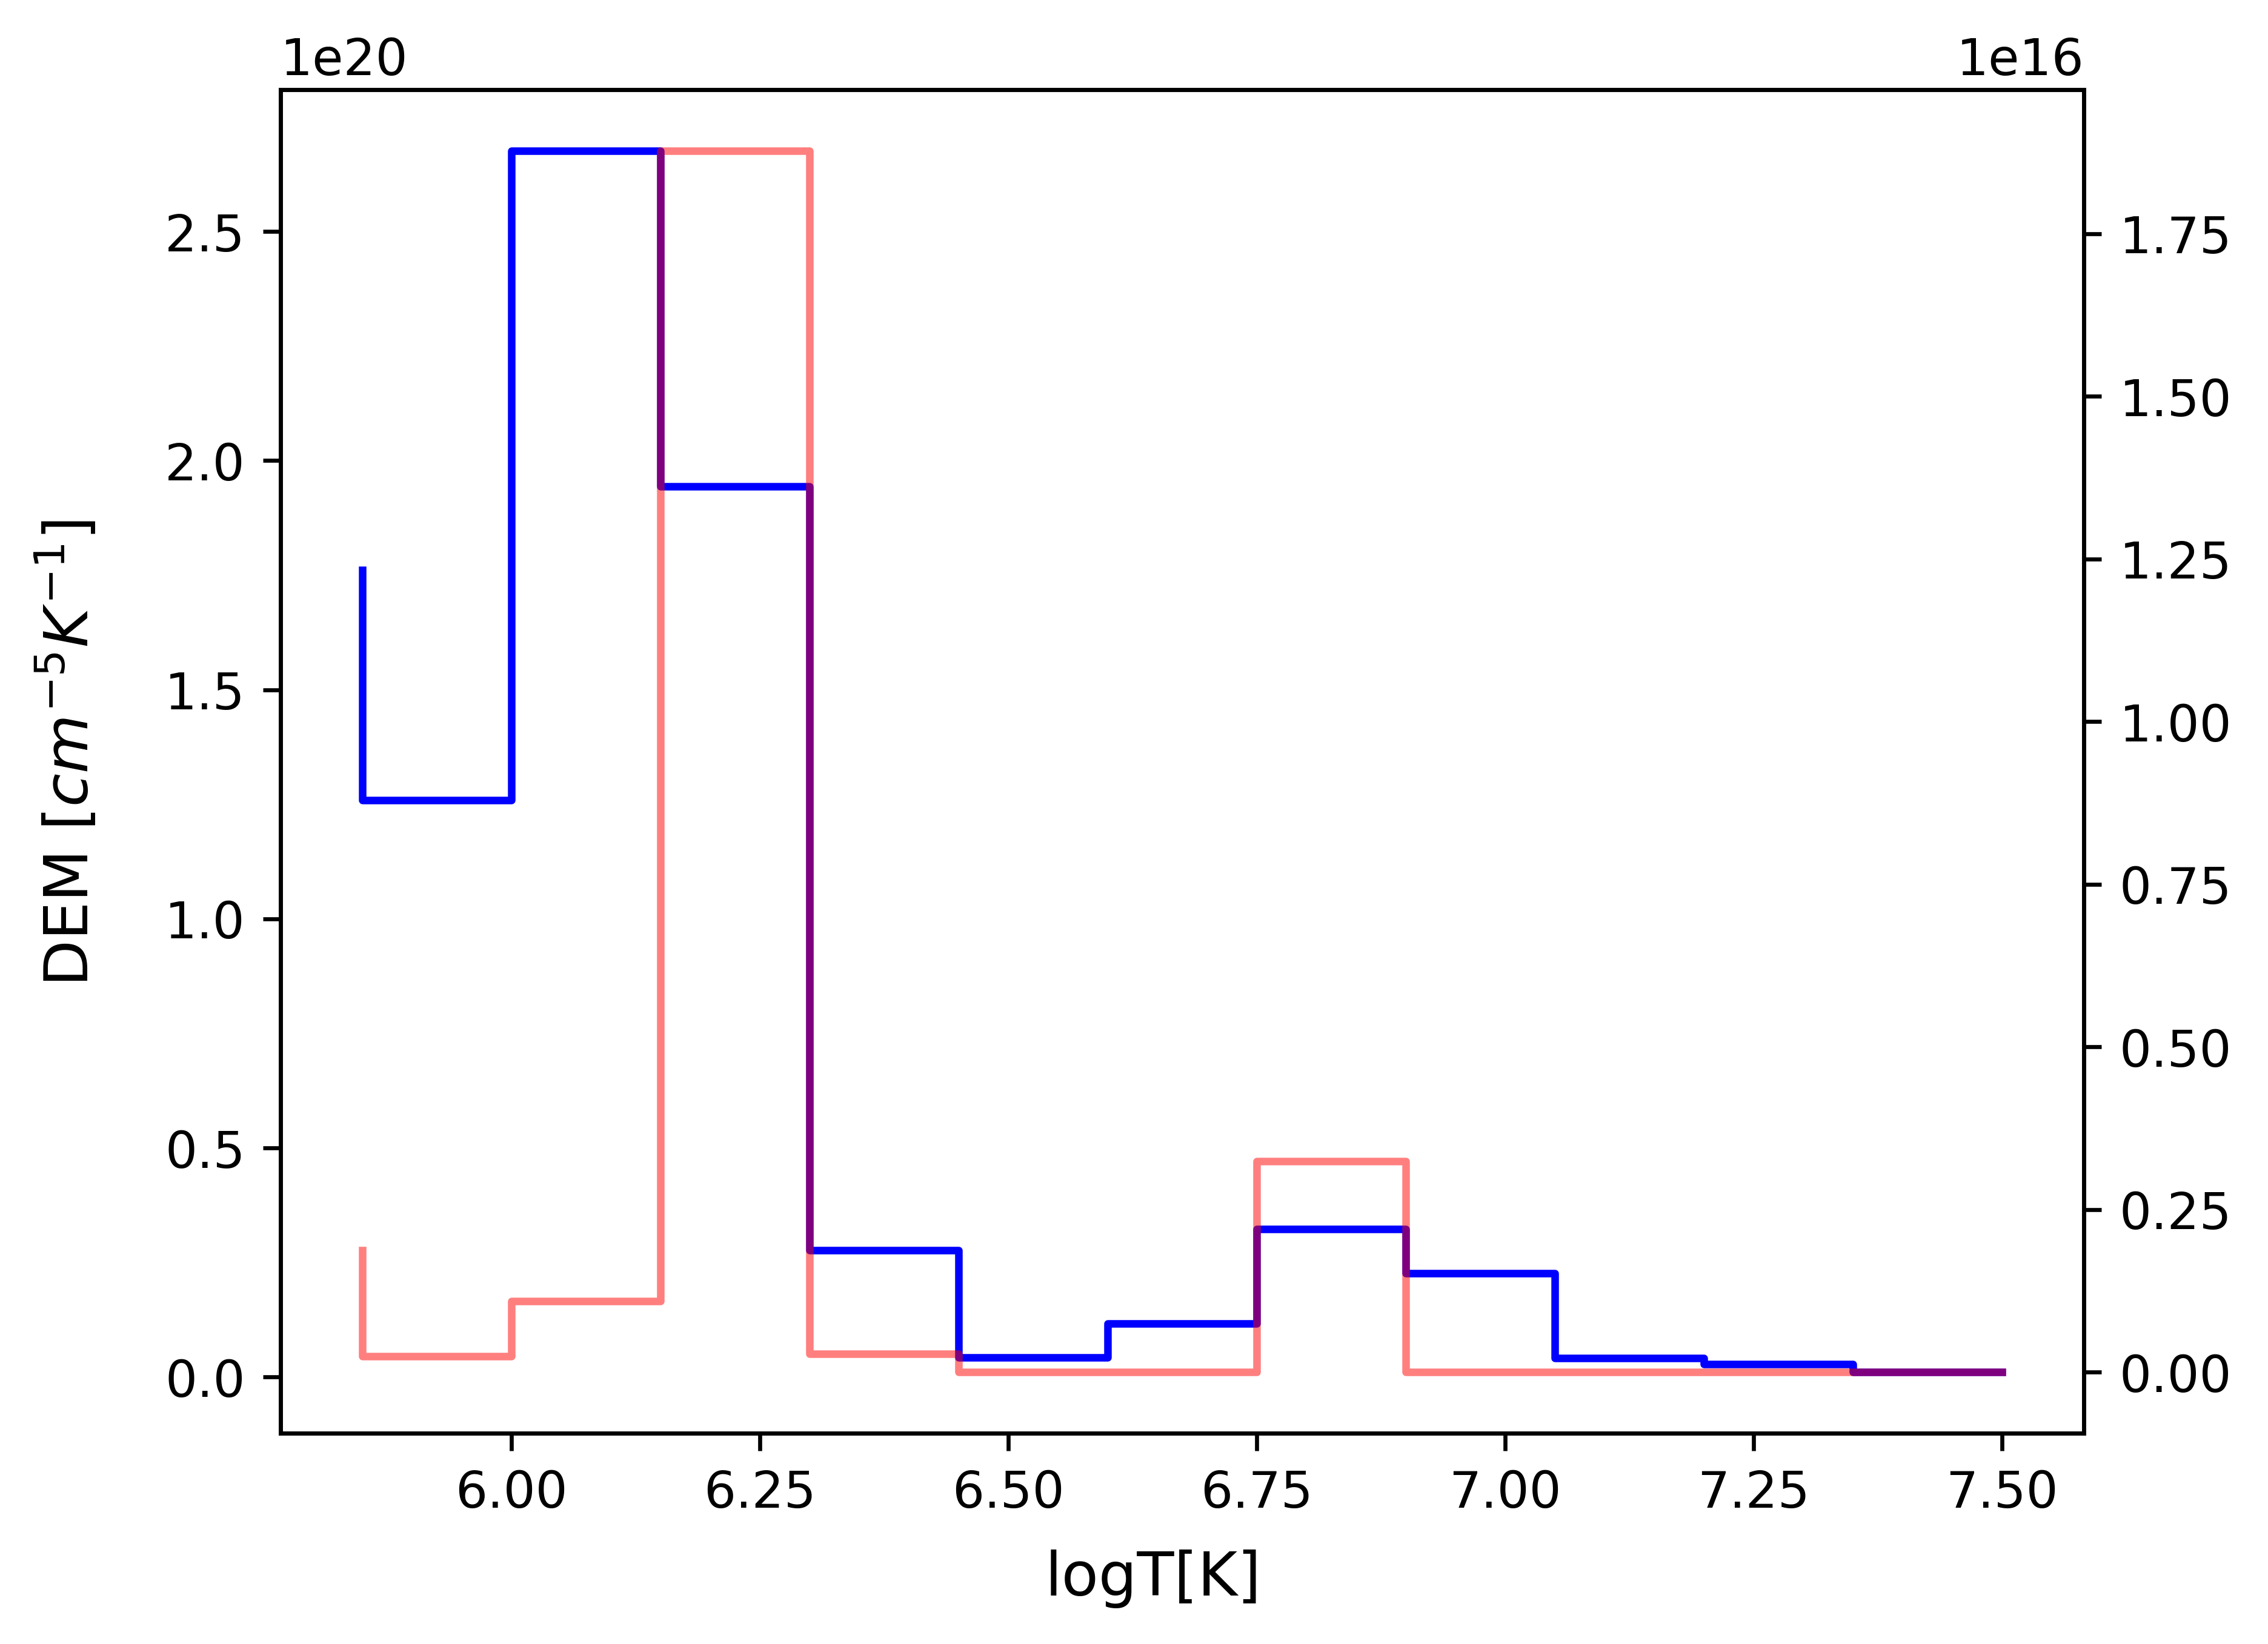
\includegraphics[width=\textwidth]{images/dem_profile_during_event_2011_aug_04.png}
        \caption{During event (04:11 UT)}
    \end{subfigure}
    \hfill
    \begin{subfigure}[b]{0.3\textwidth}
        \centering
        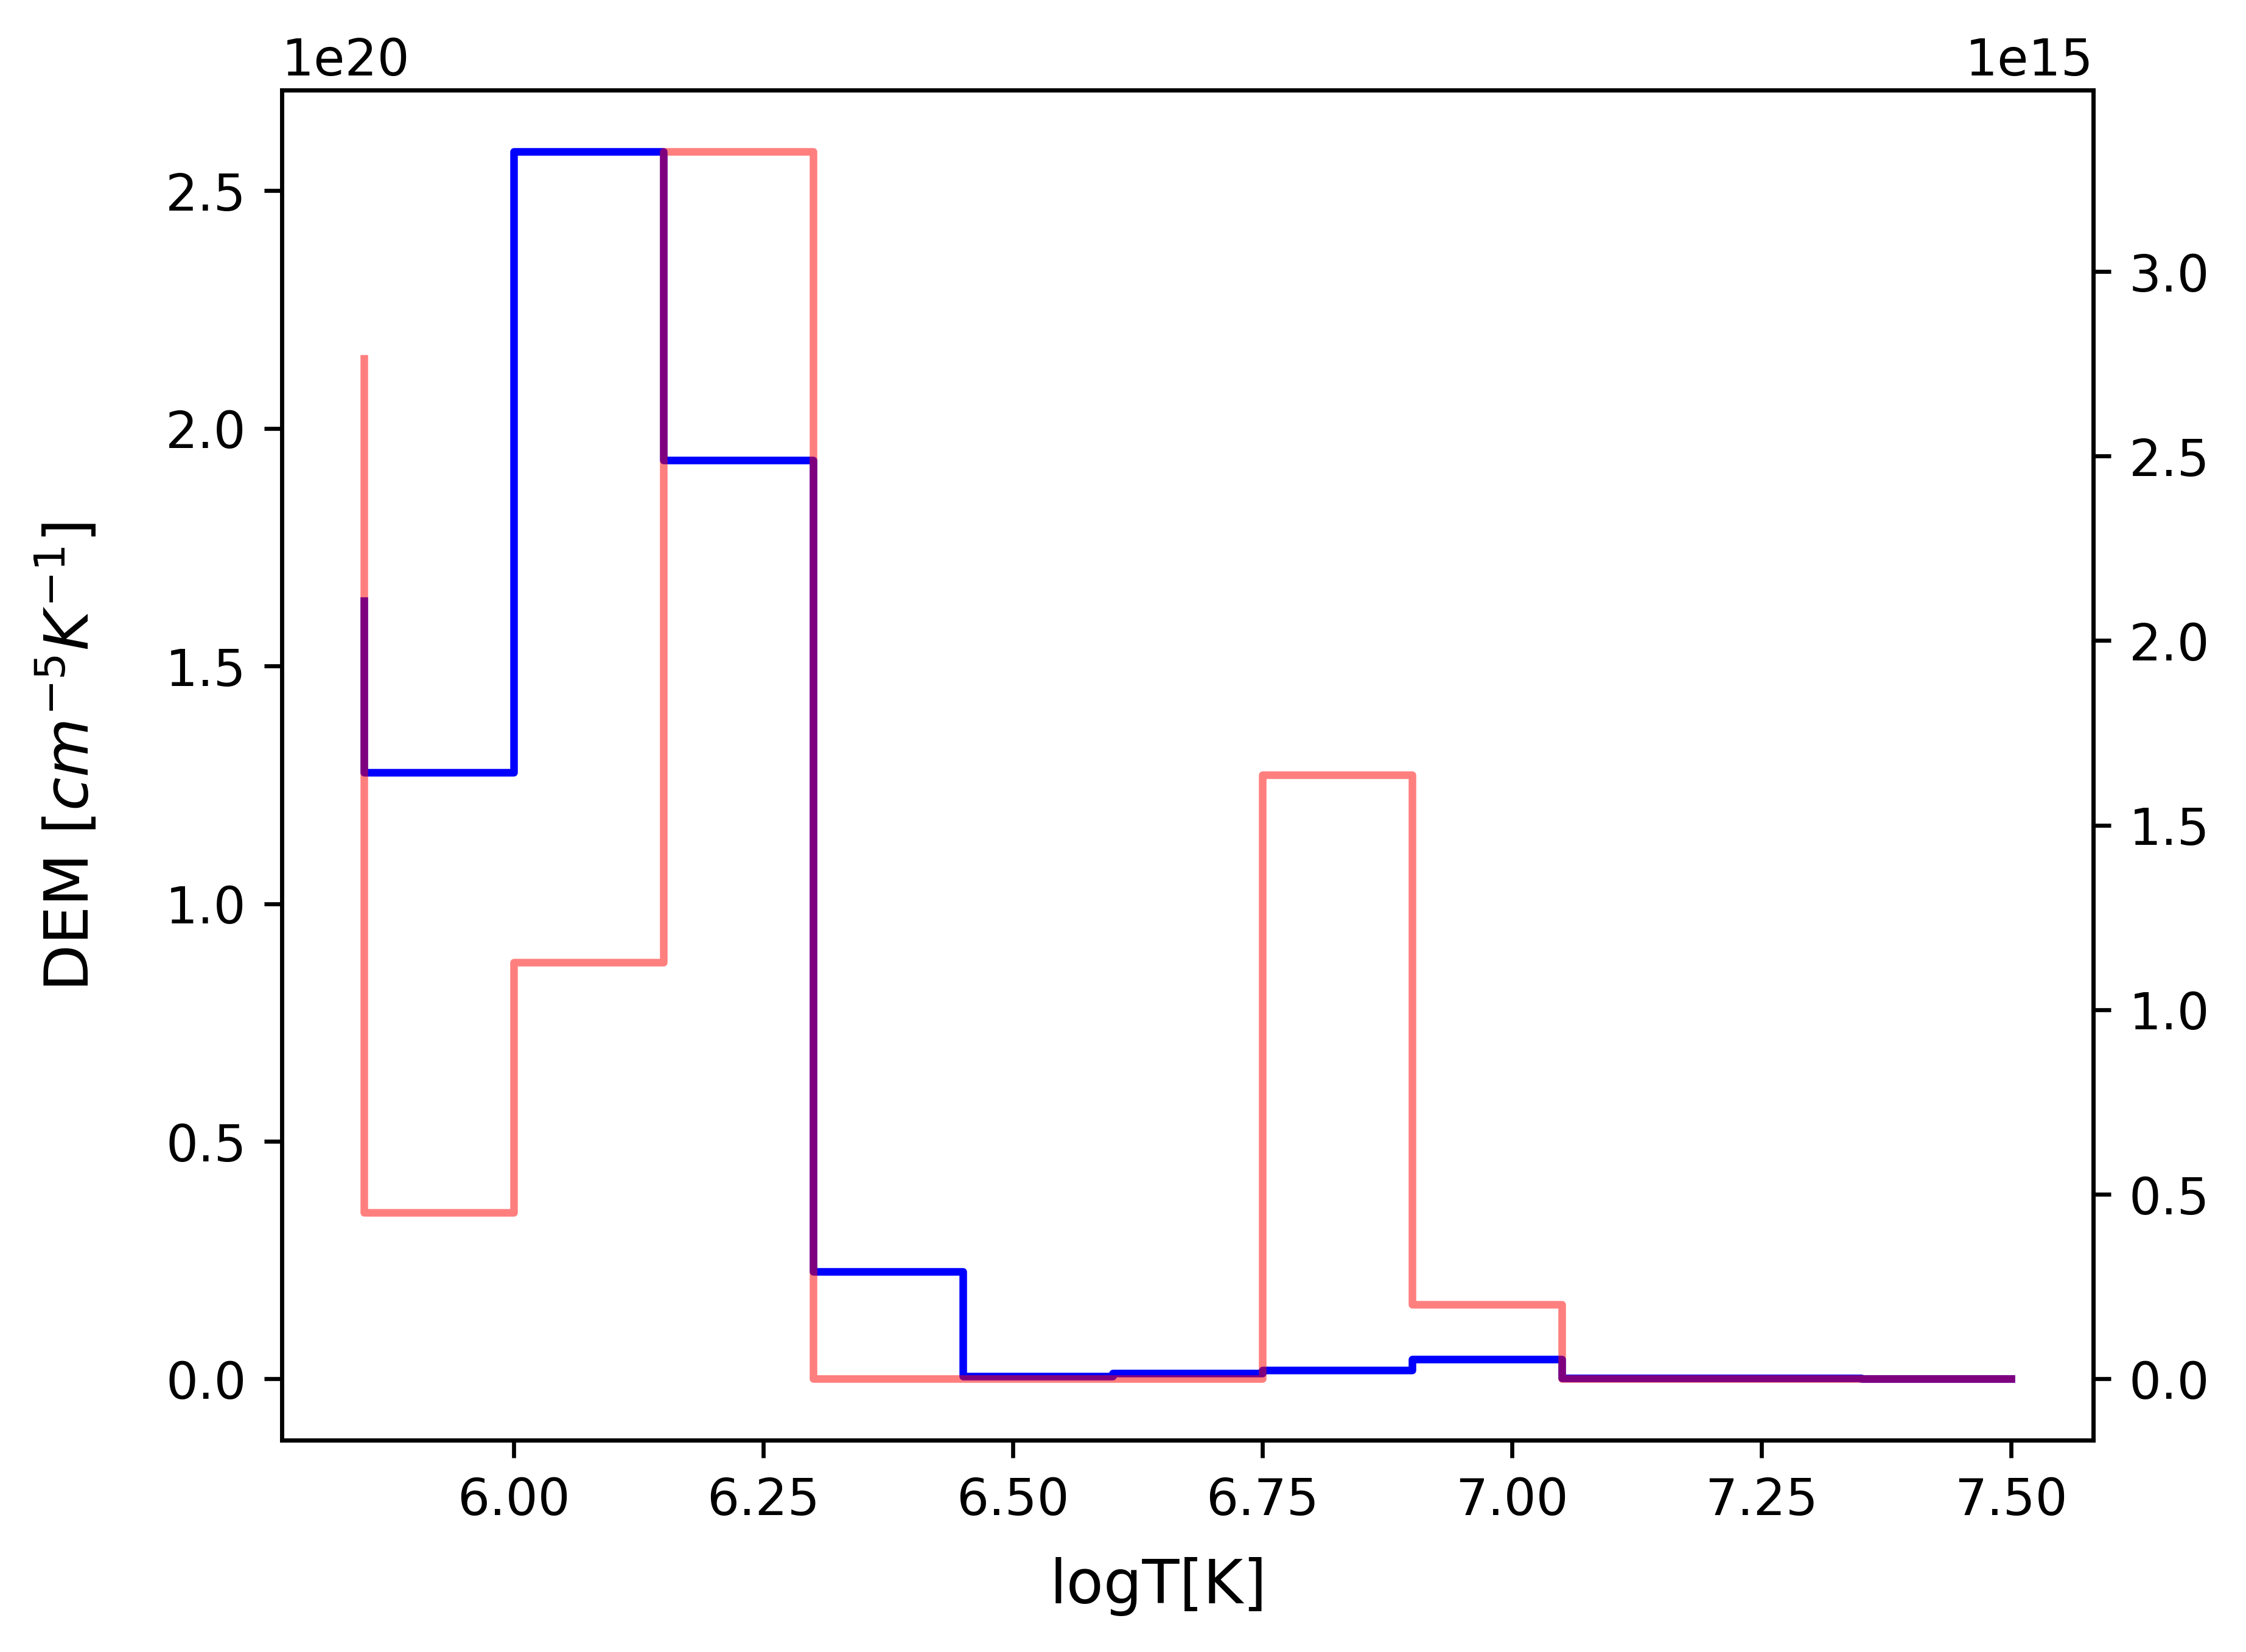
\includegraphics[width=\textwidth]{images/dem_profile_after_event_2011_aug_04.png}
        \caption{After event (10:49 UT)}
    \end{subfigure}

    \caption[DEM profile for \nth{4} August 2011 event]{DEM profile before, during and after the flaring event of \nth{4} August 2011. The red and blue curves correspond to point source and full disk source respectively.}
    \label{fig:dem_pro_aug_04_2011}
\end{figure}


\begin{figure}[h!]

    \begin{subfigure}[b]{0.3\textwidth}
        \centering
        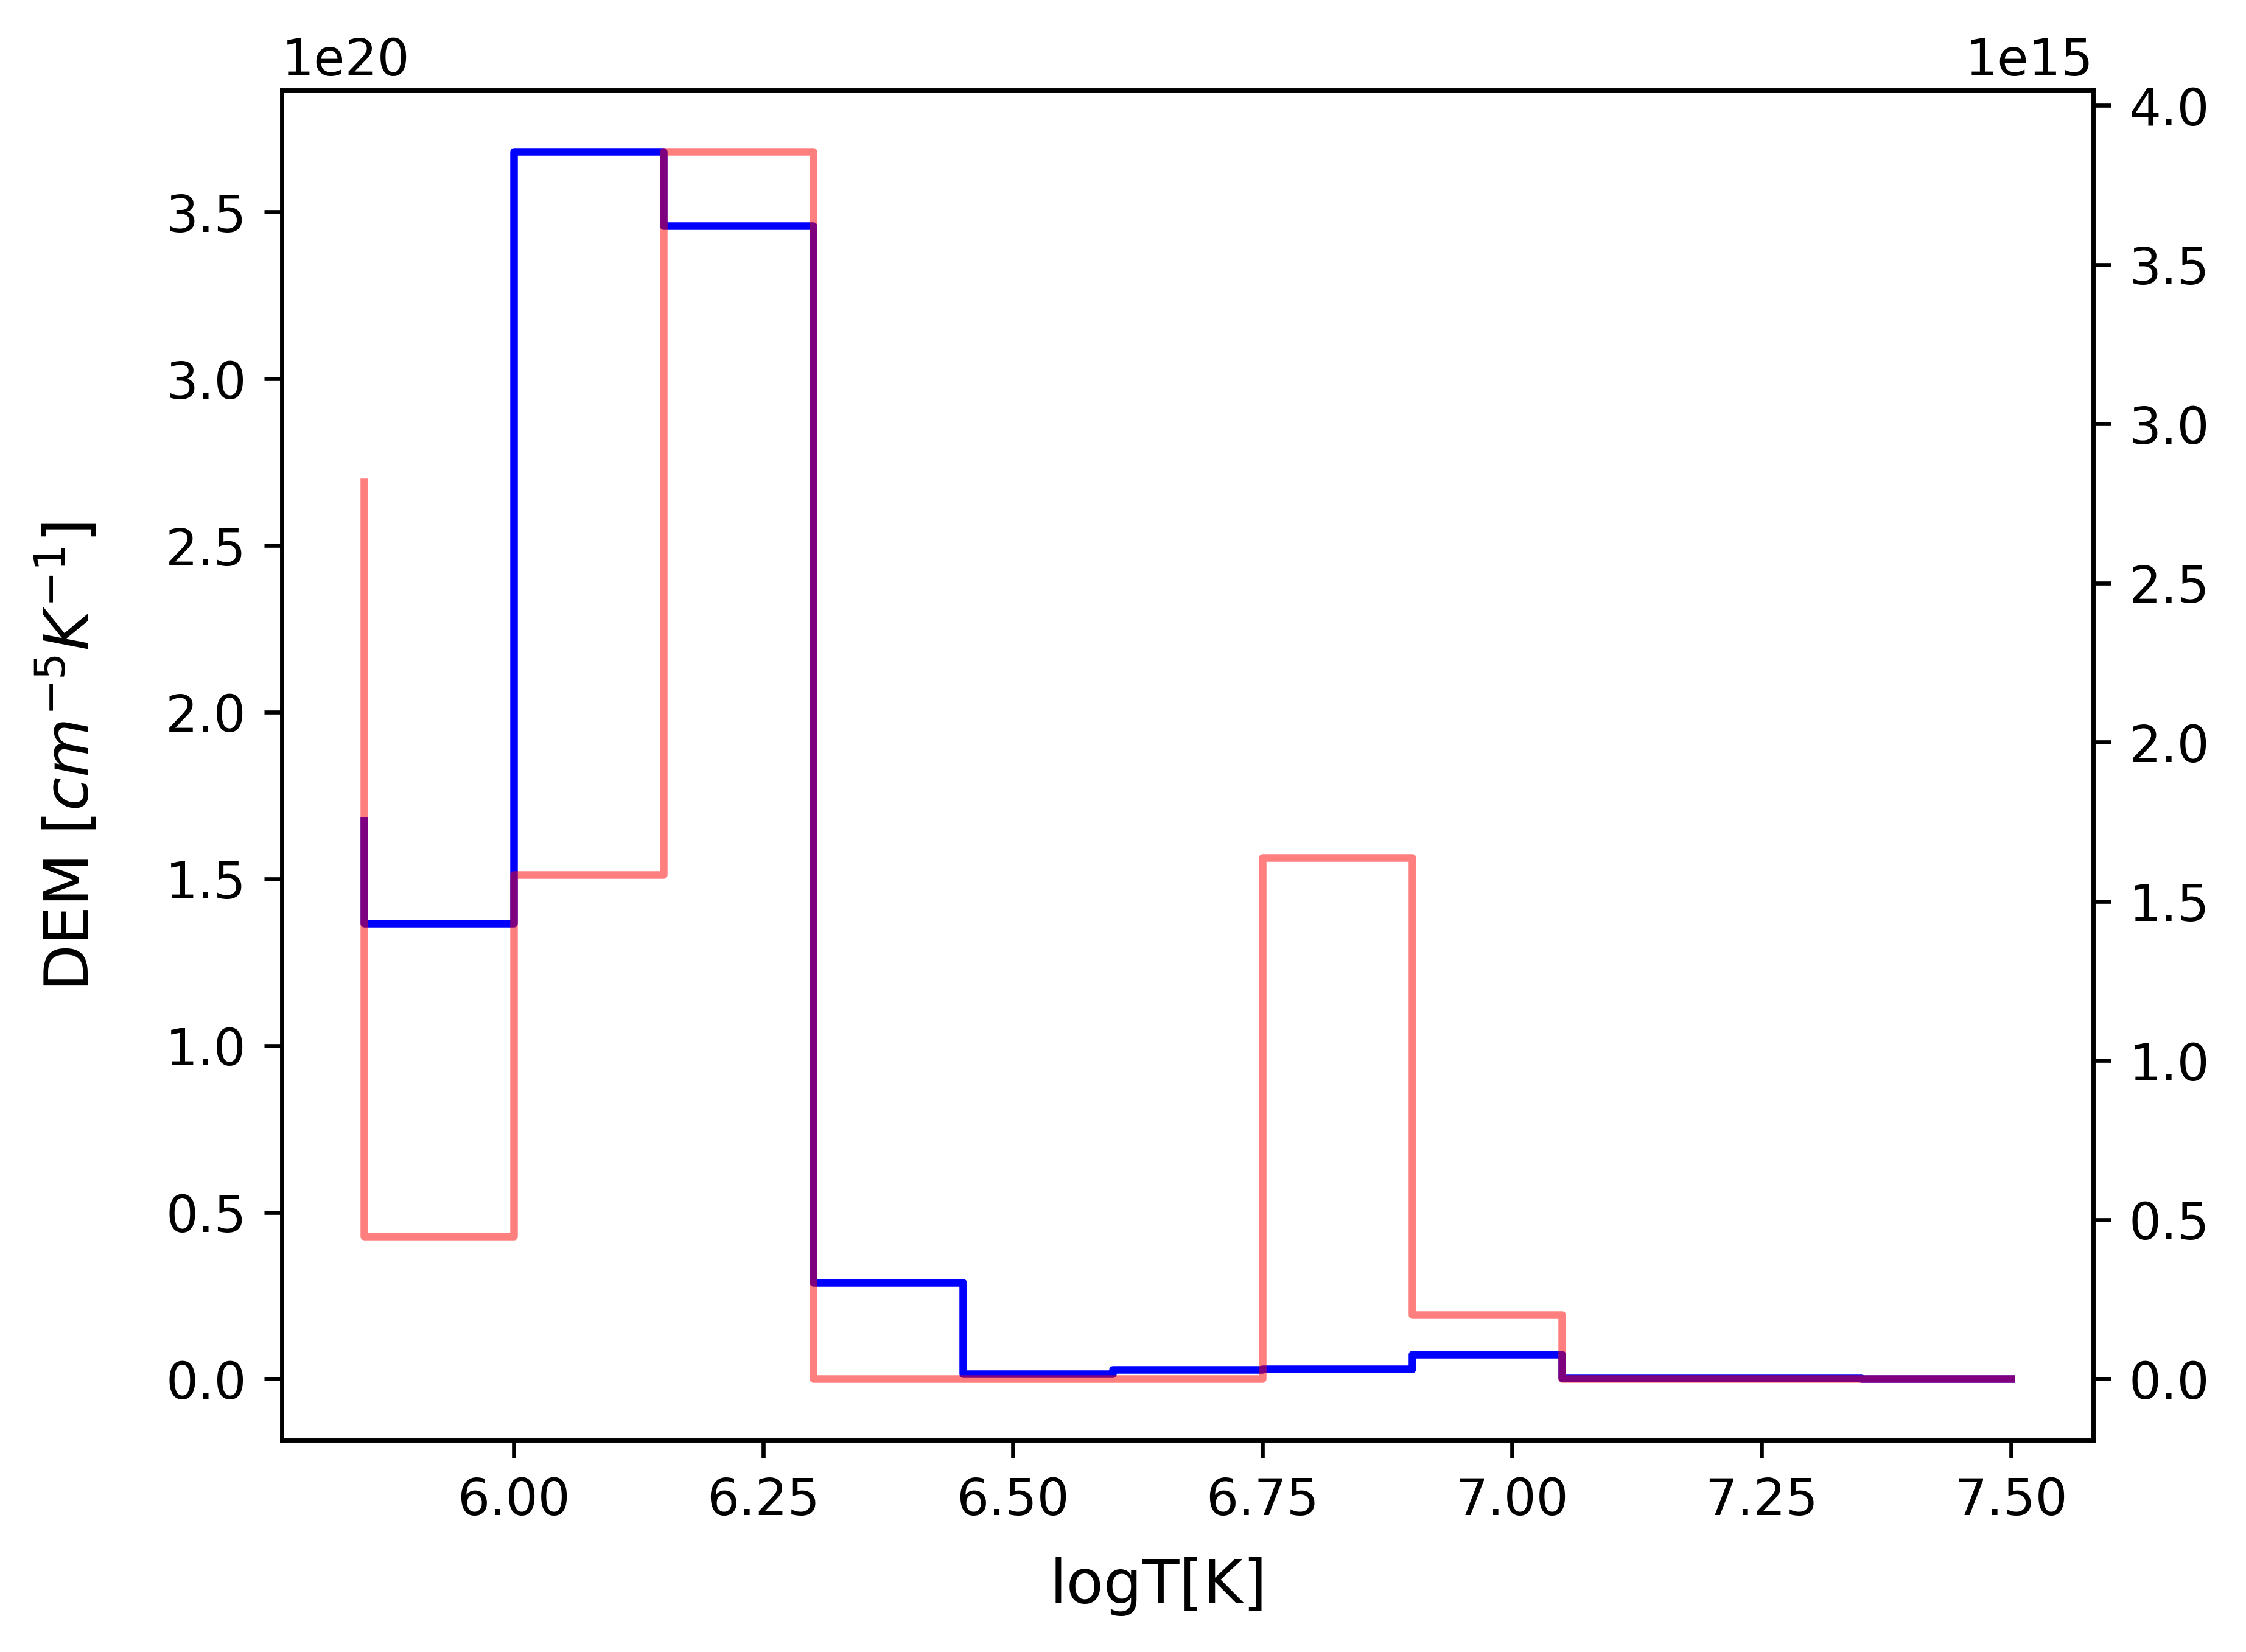
\includegraphics[width=\textwidth]{images/dem_profile_before_event_2012_aug_31.png}
        \caption{Before event (17:19 UT)}
    \end{subfigure}
    \hfill
    \begin{subfigure}[b]{0.3\textwidth}
        \centering
        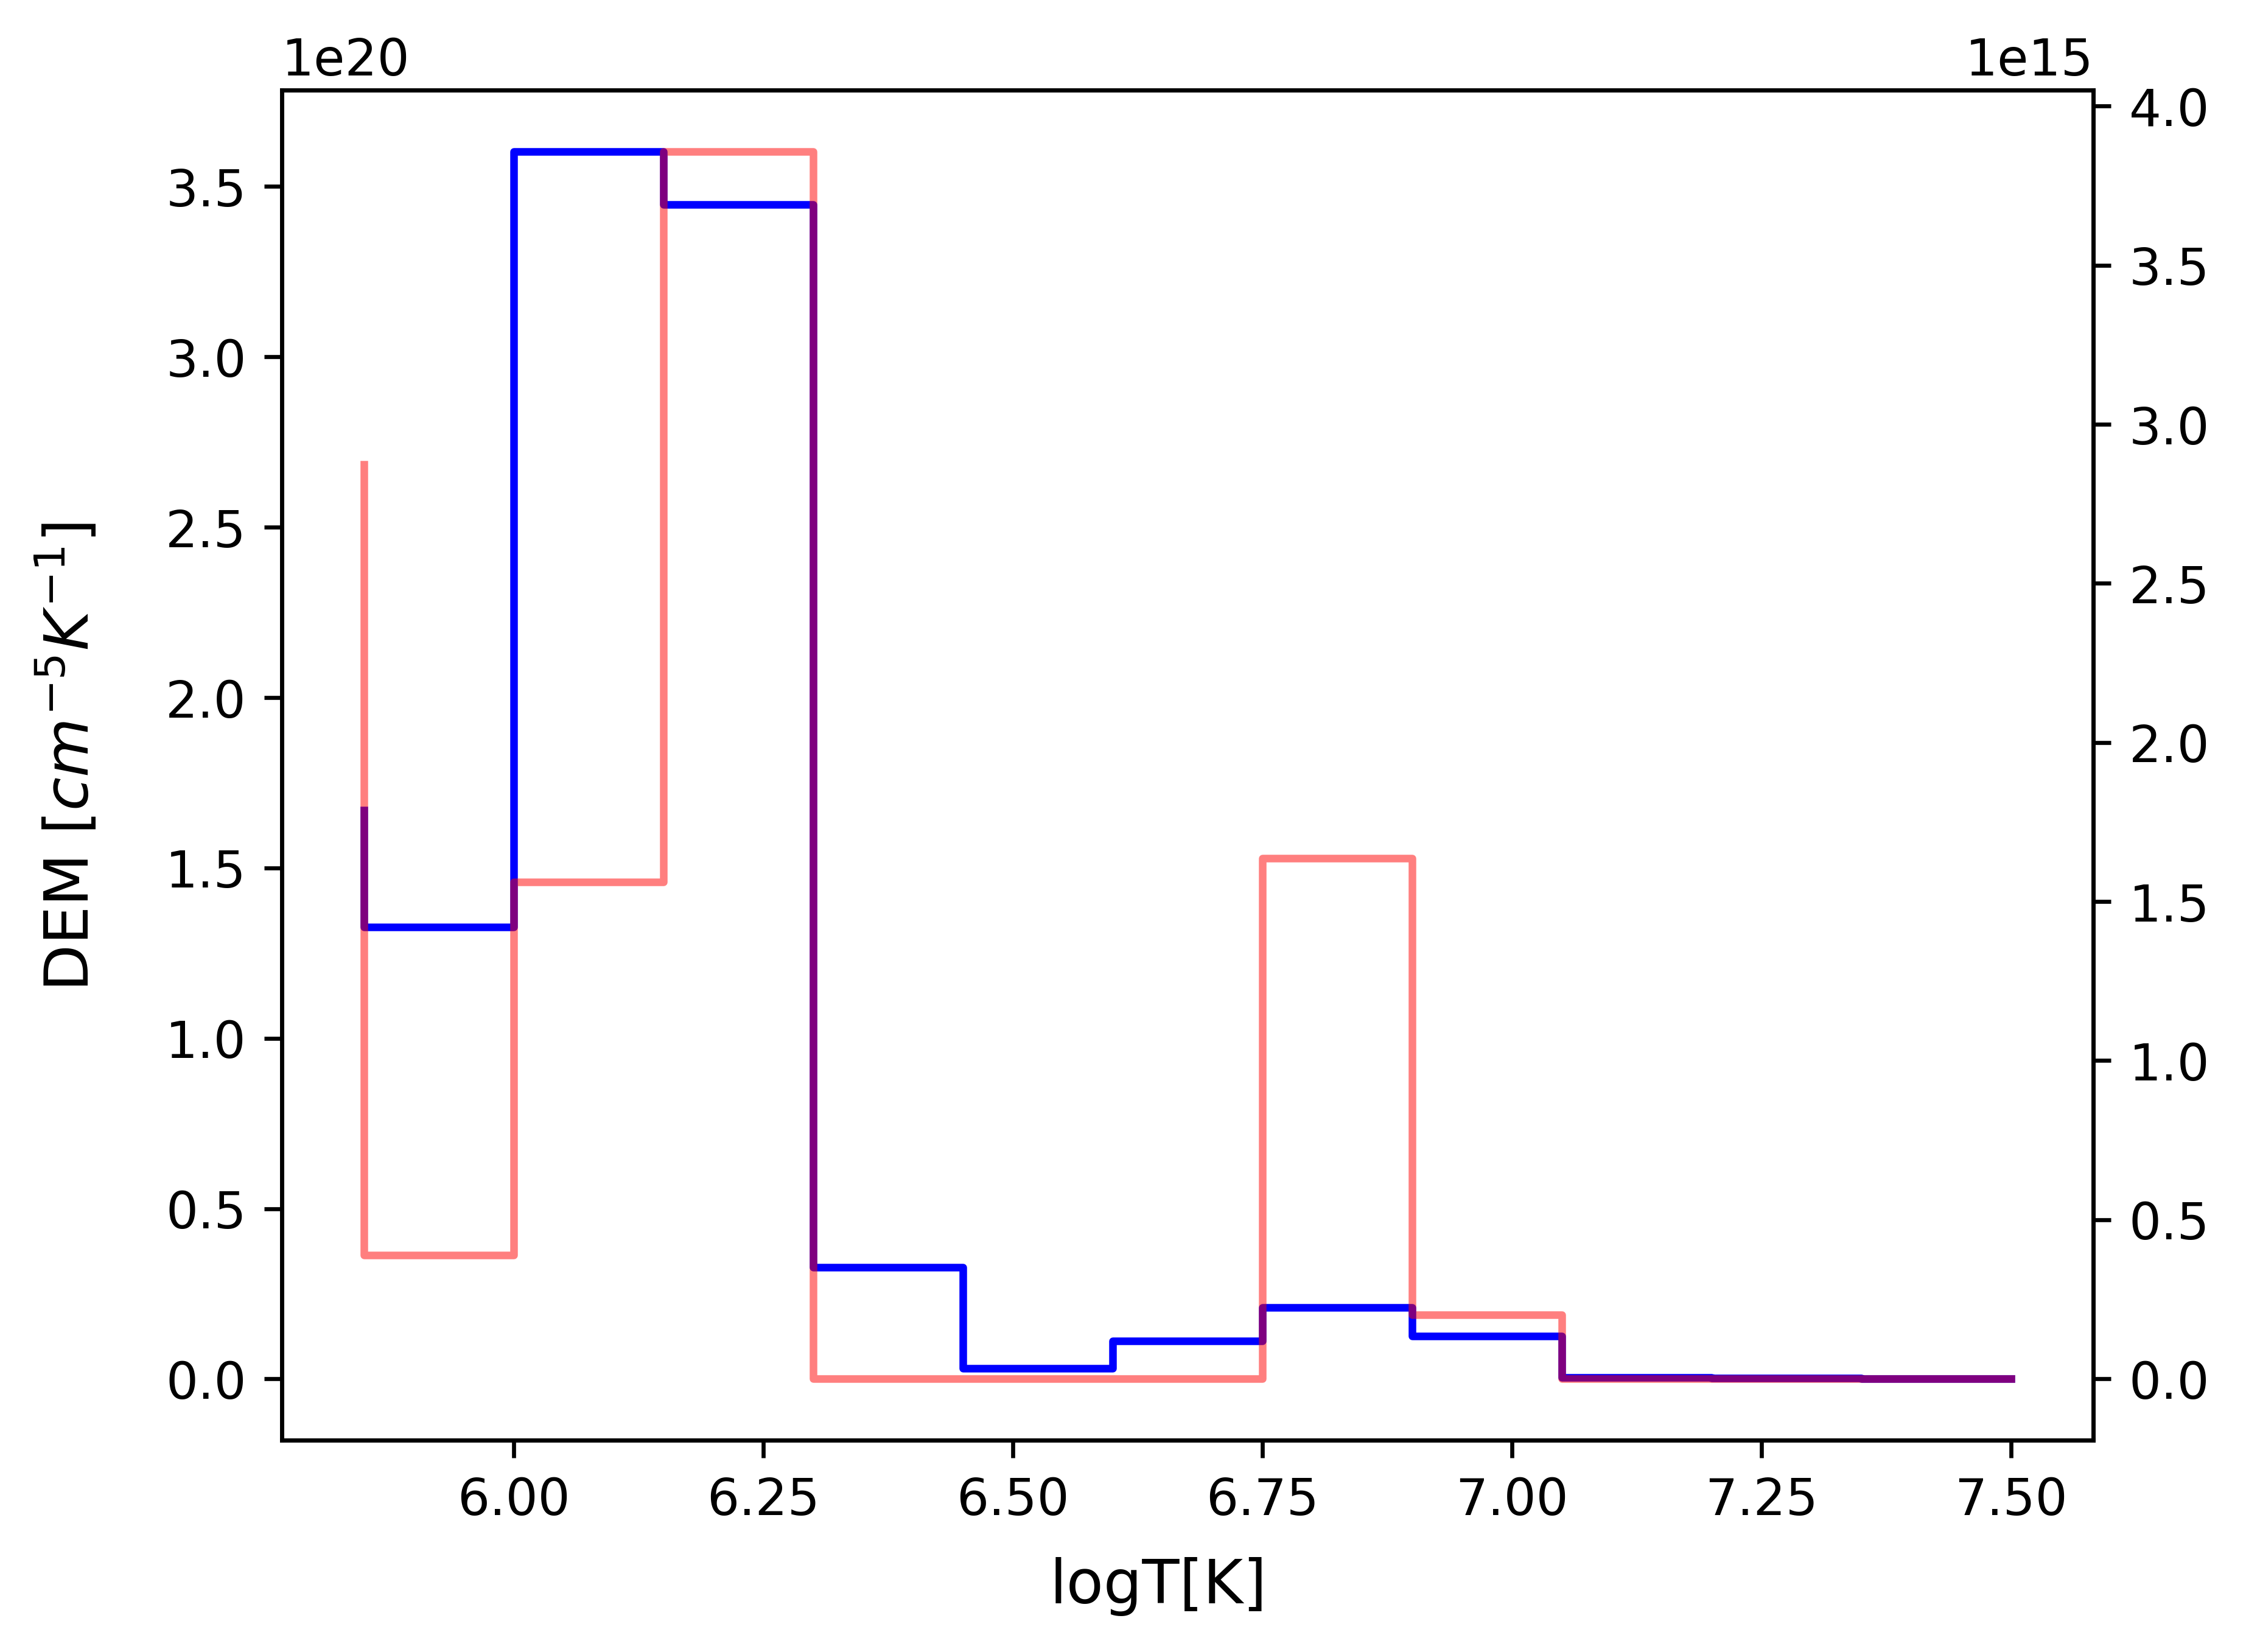
\includegraphics[width=\textwidth]{images/dem_profile_during_event_2012_aug_31.png}
        \caption{During event (20:01 UT)}
    \end{subfigure}
    \hfill
    \begin{subfigure}[b]{0.3\textwidth}
        \centering
        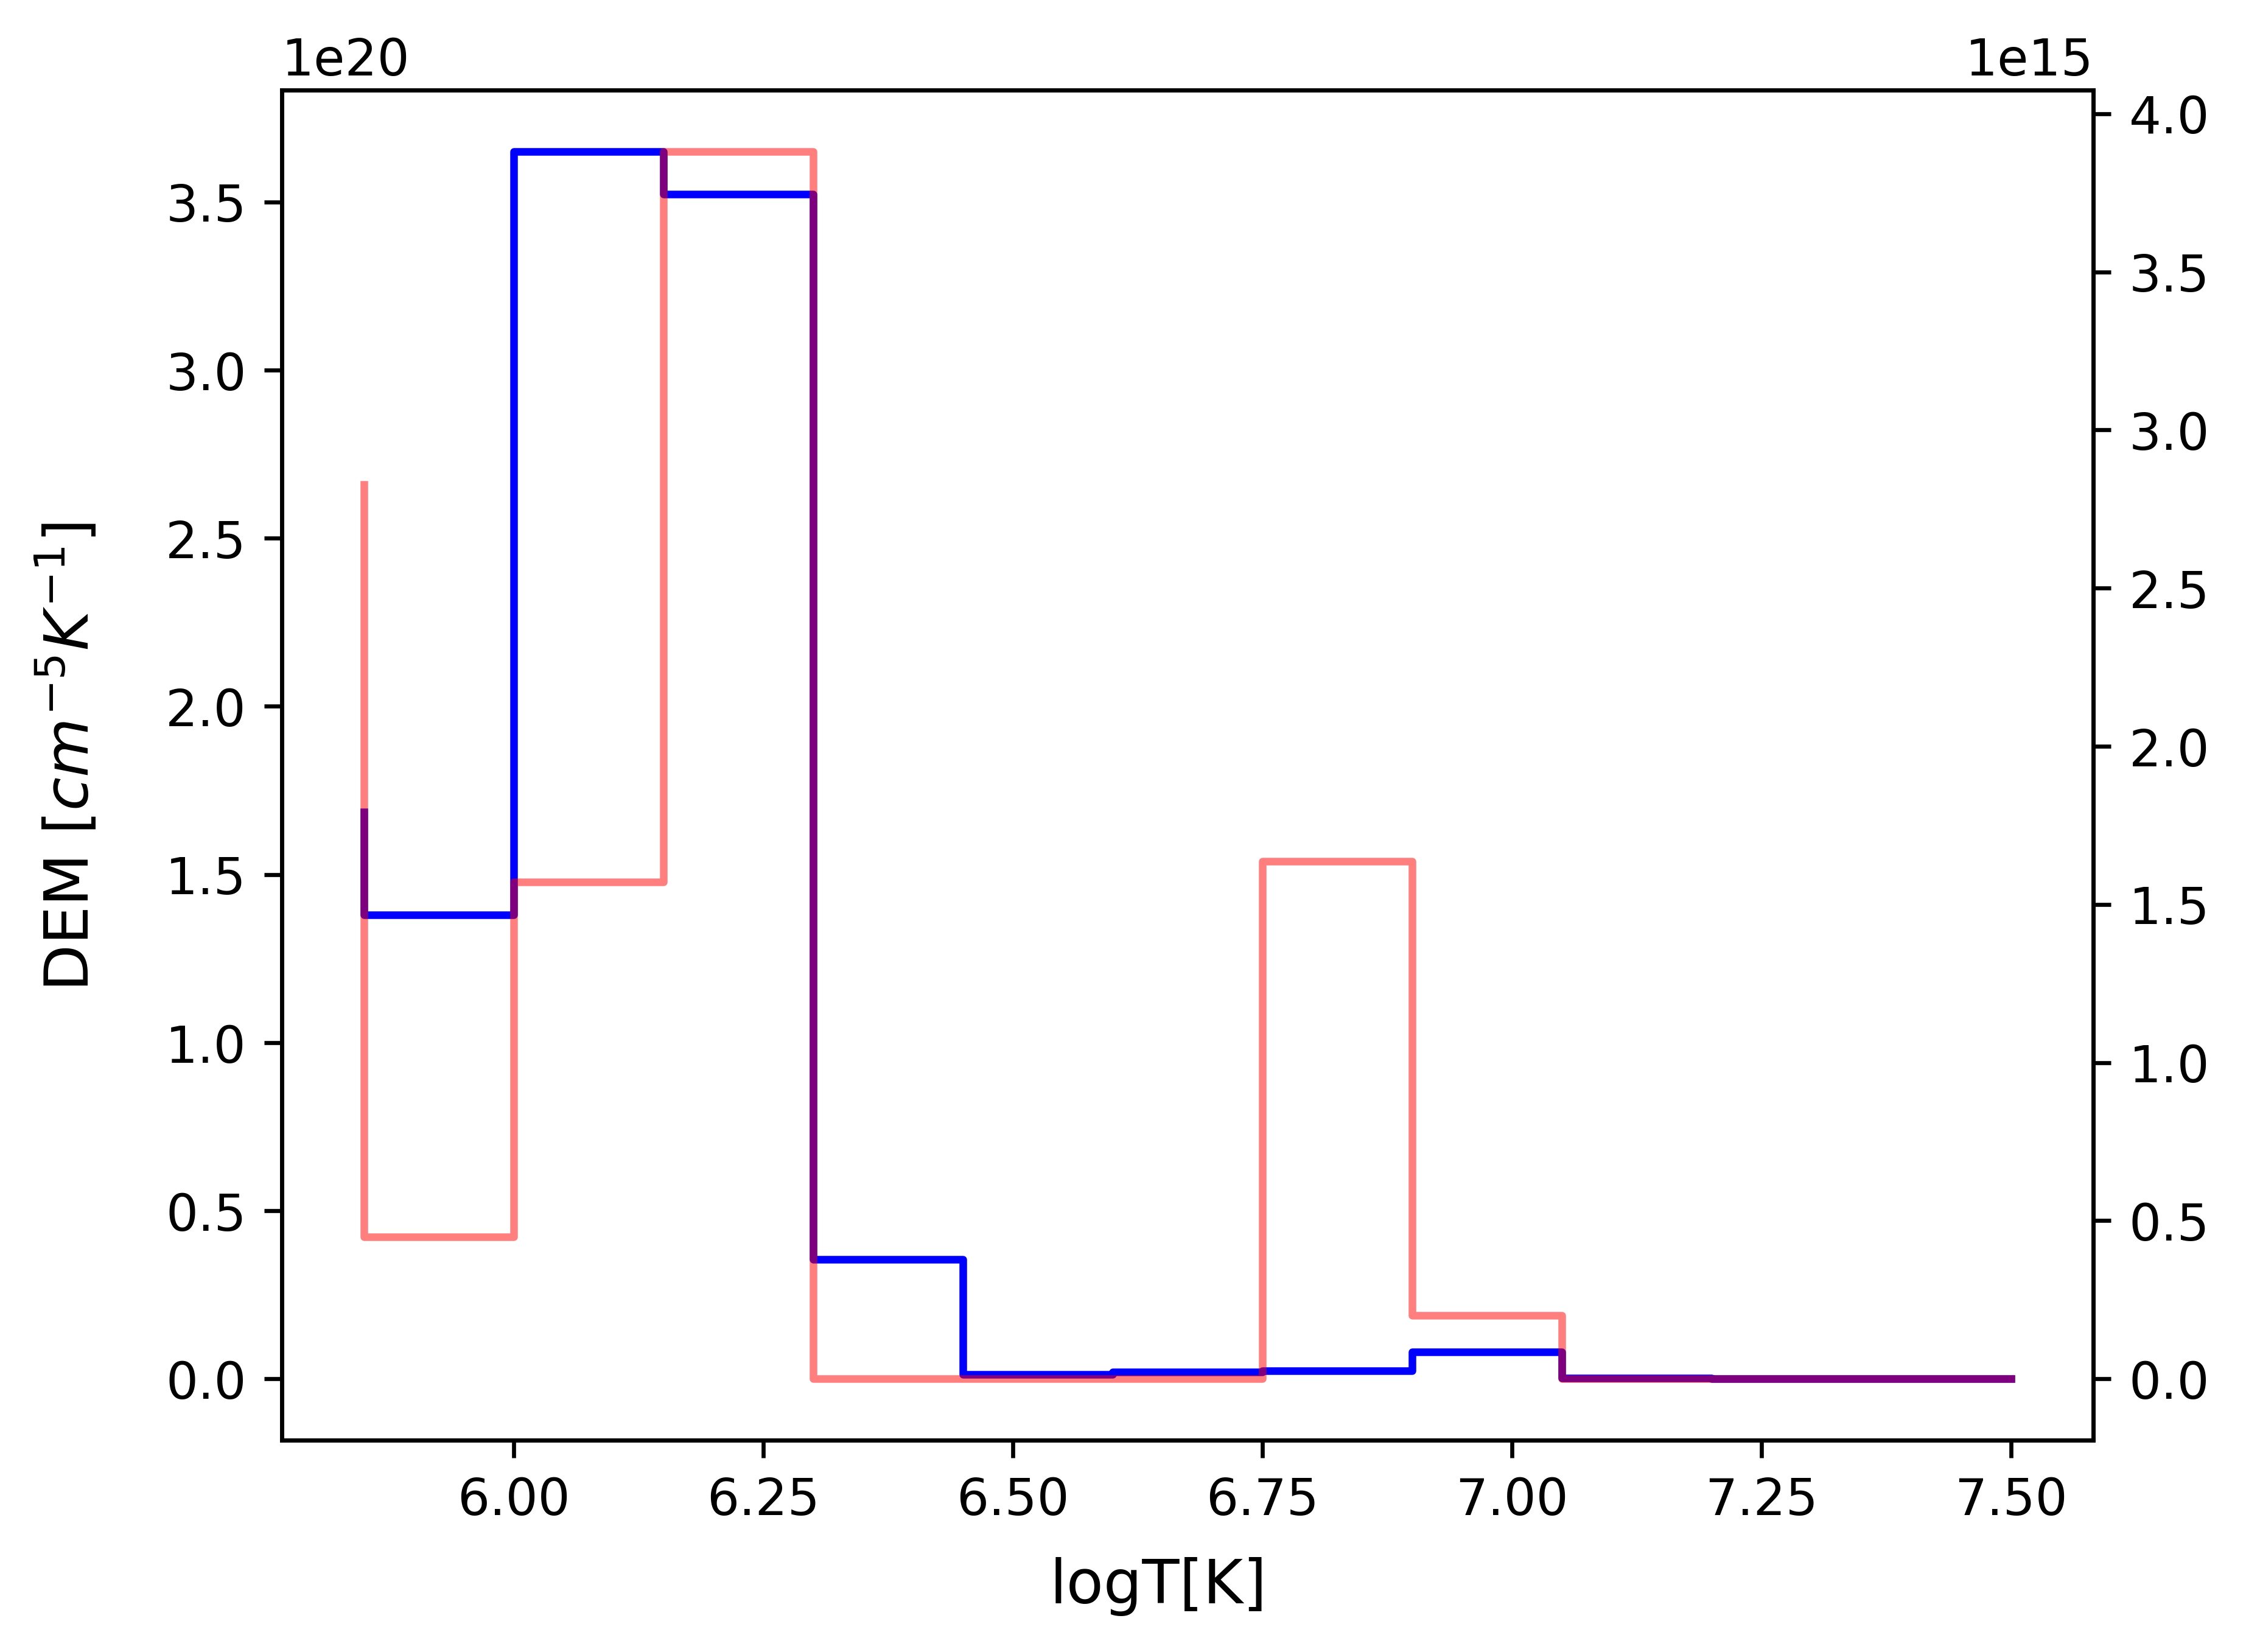
\includegraphics[width=\textwidth]{images/dem_profile_after_event_2012_aug_31.png}
        \caption{After event (\nth{1} September 2011 03:57 UT)}
    \end{subfigure}

    \caption[DEM profile for \nth{31} August 2012 Event]{DEM profile before, during and after the flaring event of \nth{31} August 2012. The red and blue curves correspond to point source and full disk source respectively}
    \label{fig:dem_pro_aug_31_2012}
\end{figure}

\begin{figure}[h!]

    \begin{subfigure}[b]{0.3\textwidth}
        \centering
        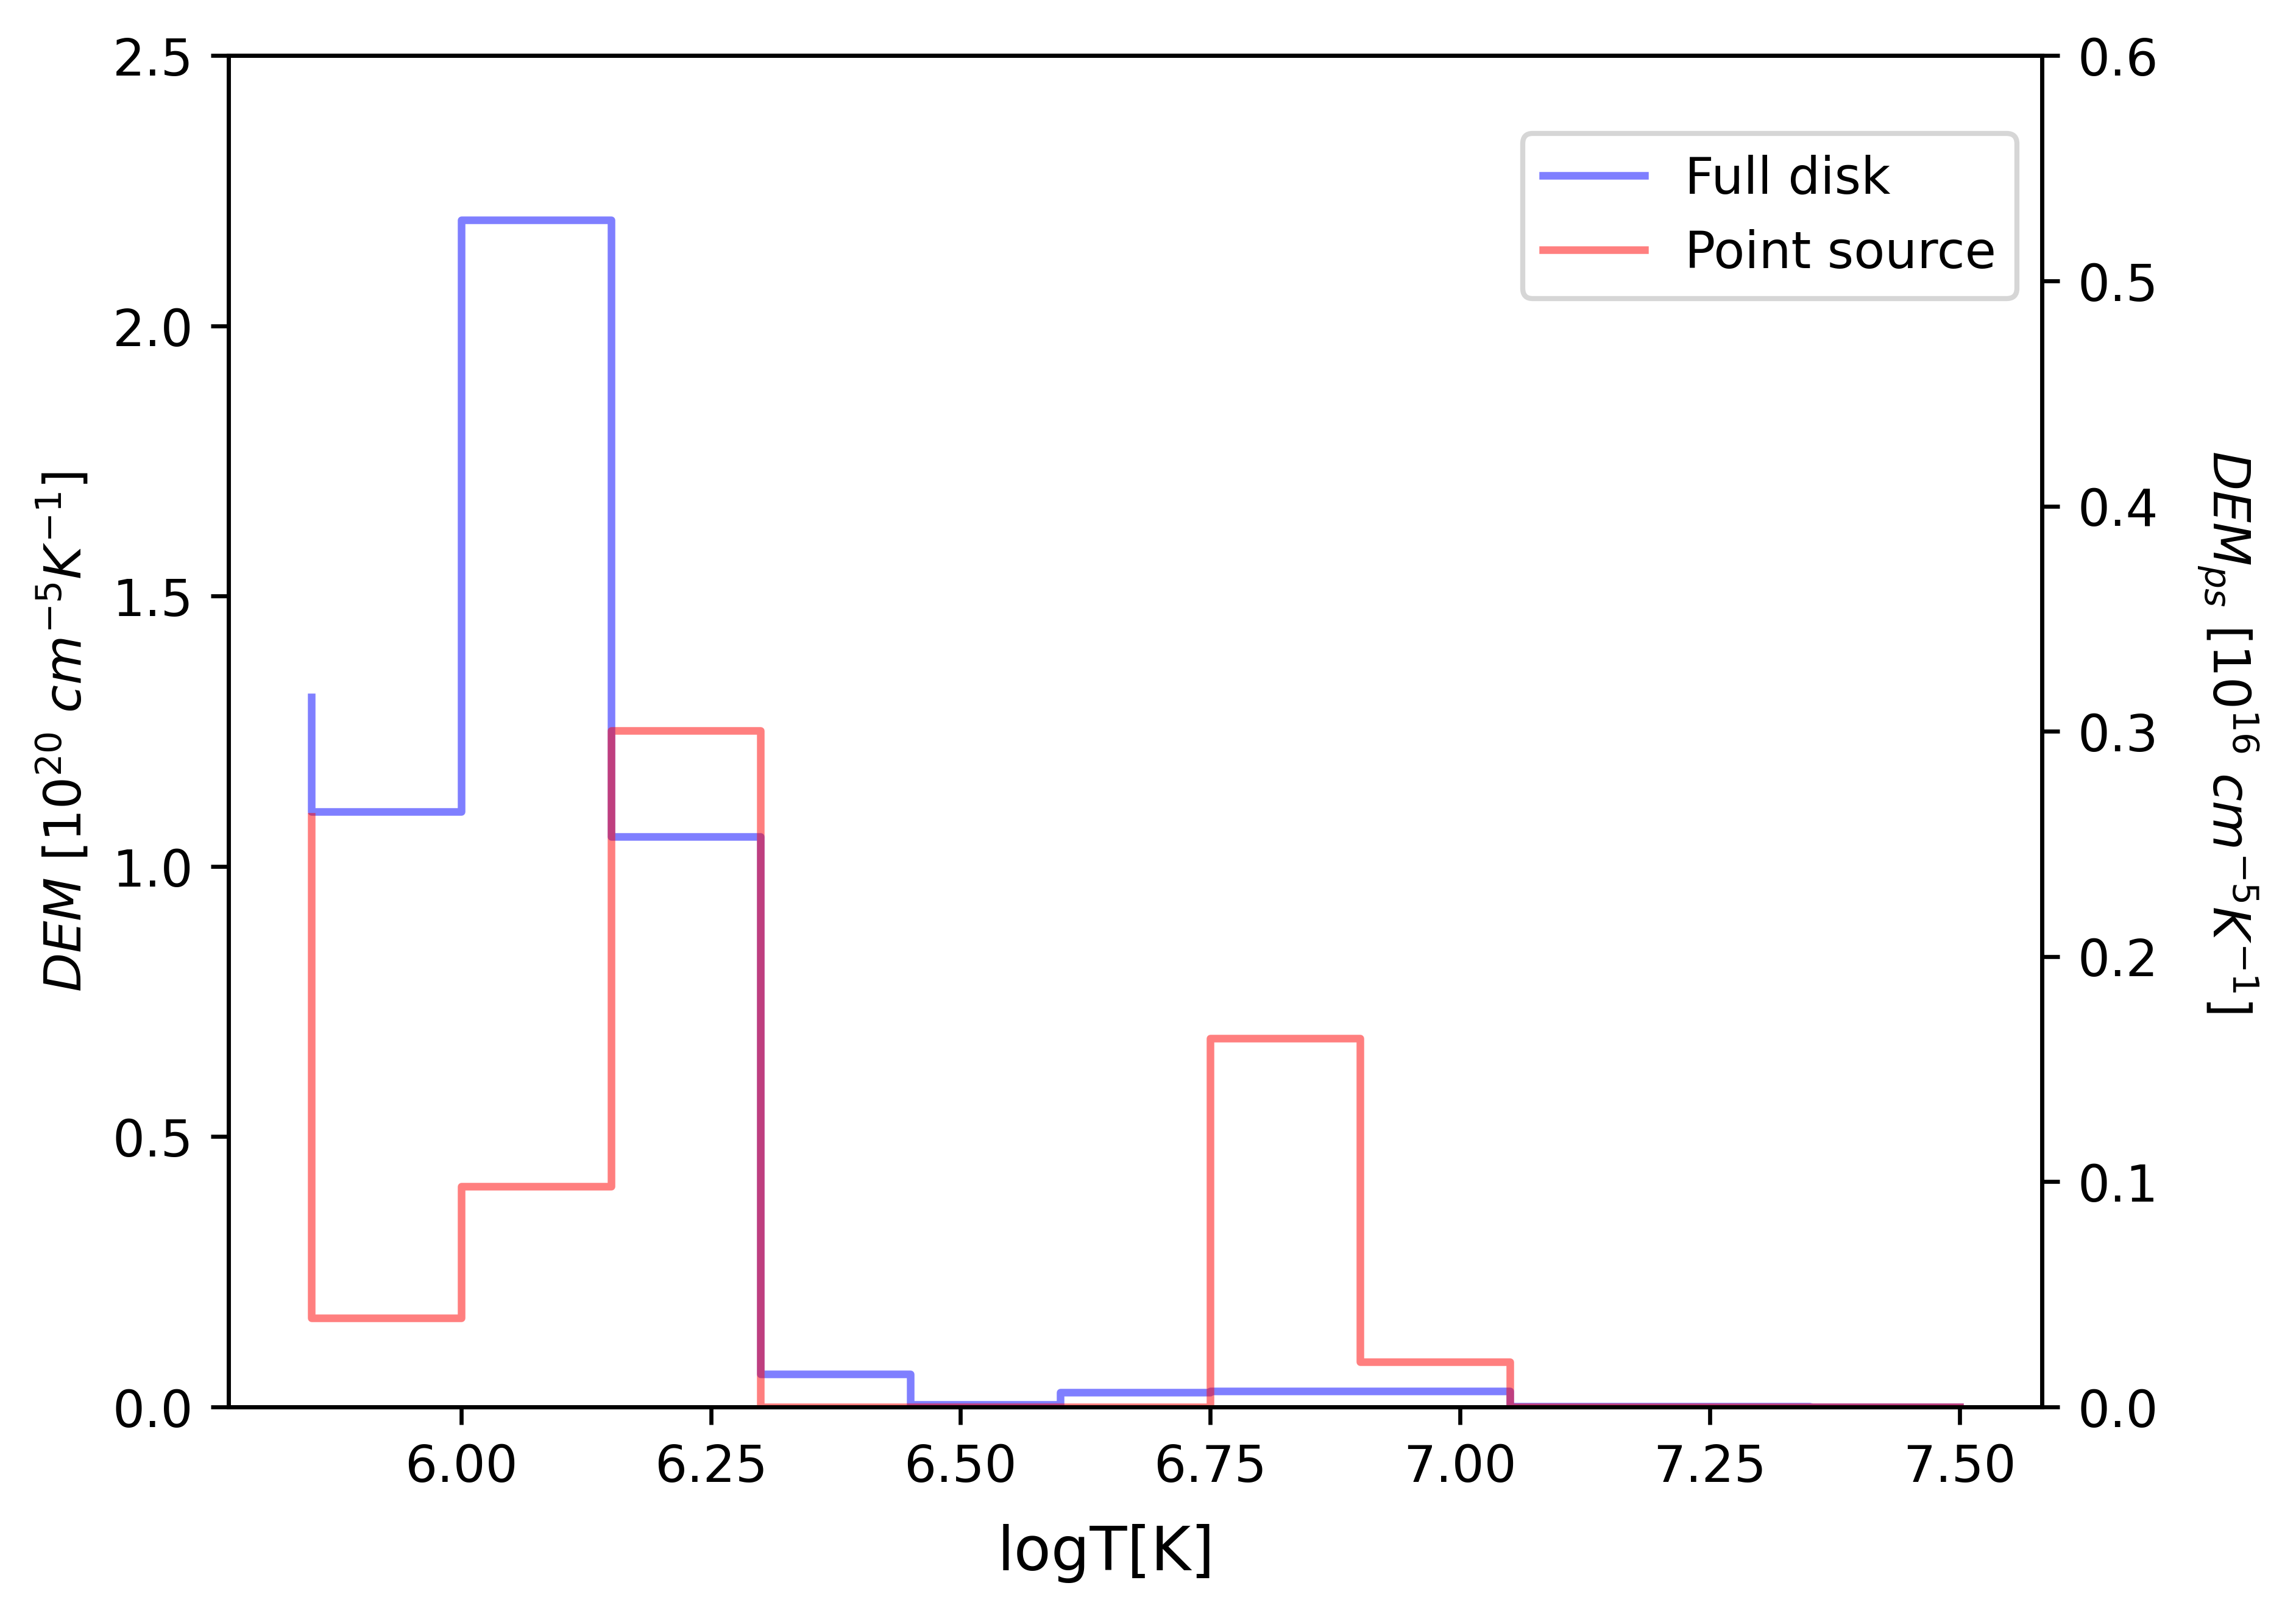
\includegraphics[width=\textwidth]{images/dem_profile_before_event_2021_oct_28.png}
        \caption{Before event (13:23 UT)}
    \end{subfigure}
    \hfill
    \begin{subfigure}[b]{0.3\textwidth}
        \centering
        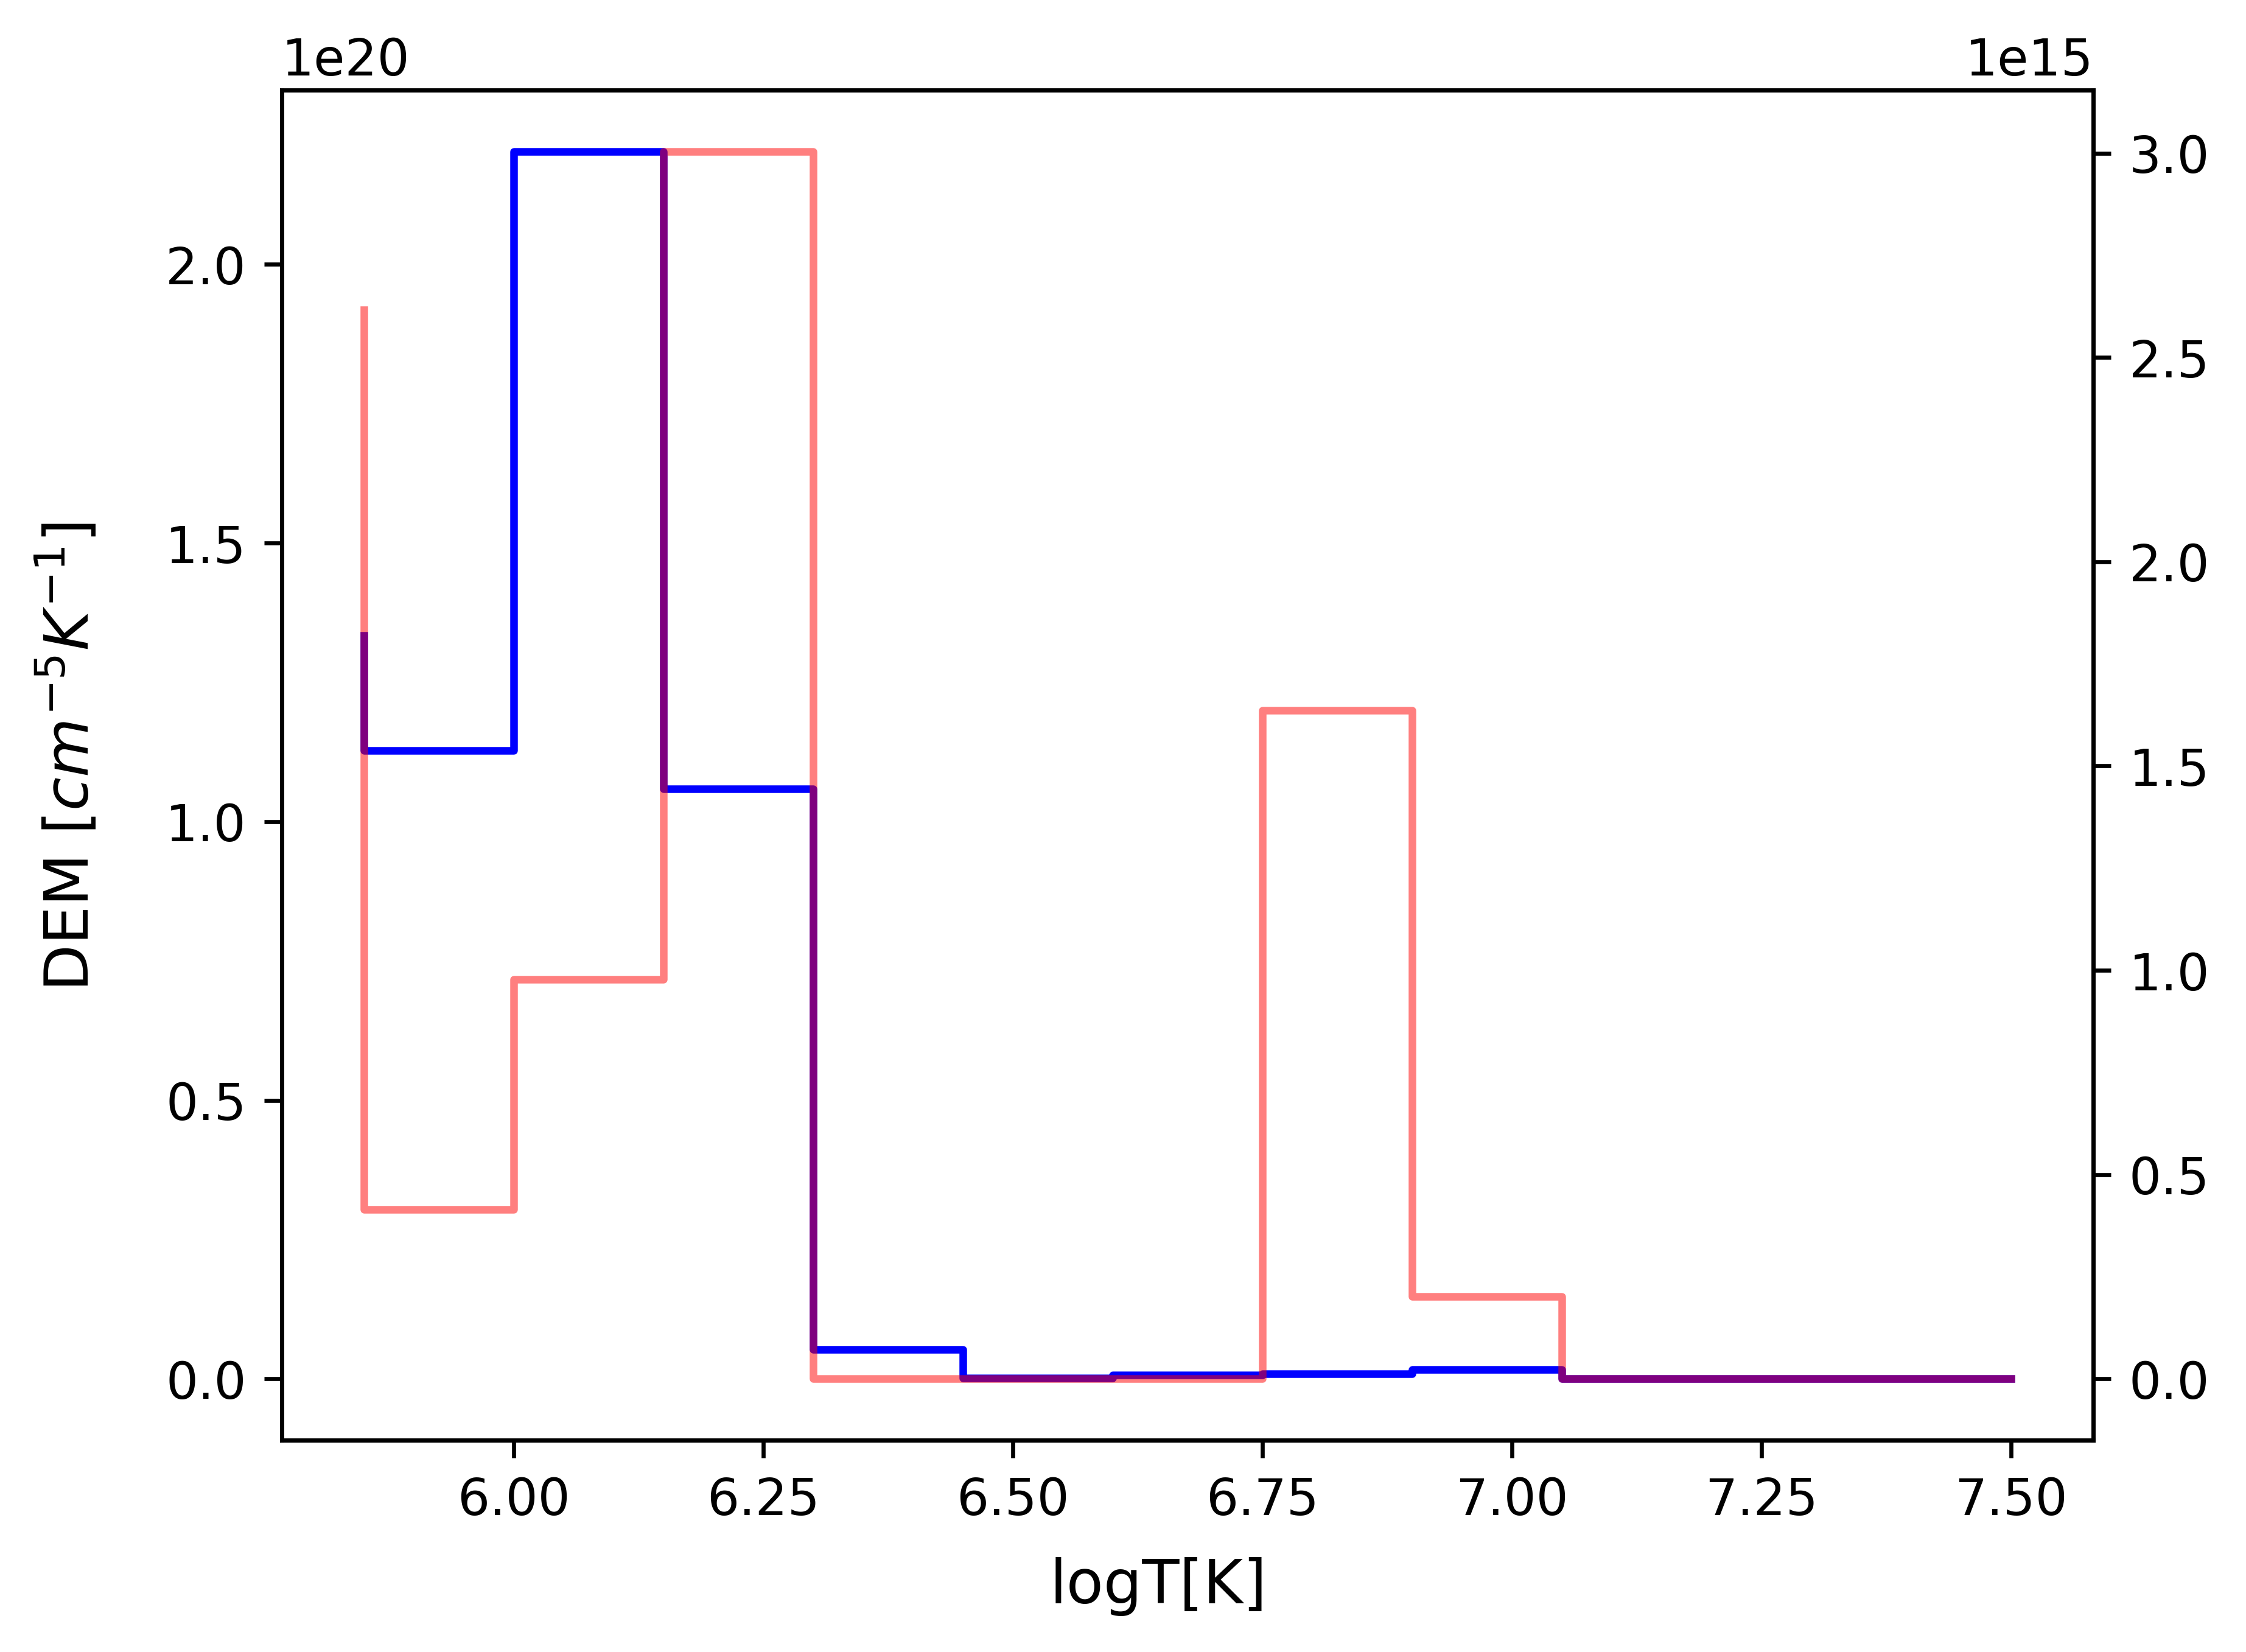
\includegraphics[width=\textwidth]{images/dem_profile_during_event_2021_oct_28.png}
        \caption{During event (15:17 UT)}
    \end{subfigure}
    \hfill
    \begin{subfigure}[b]{0.3\textwidth}
        \centering
        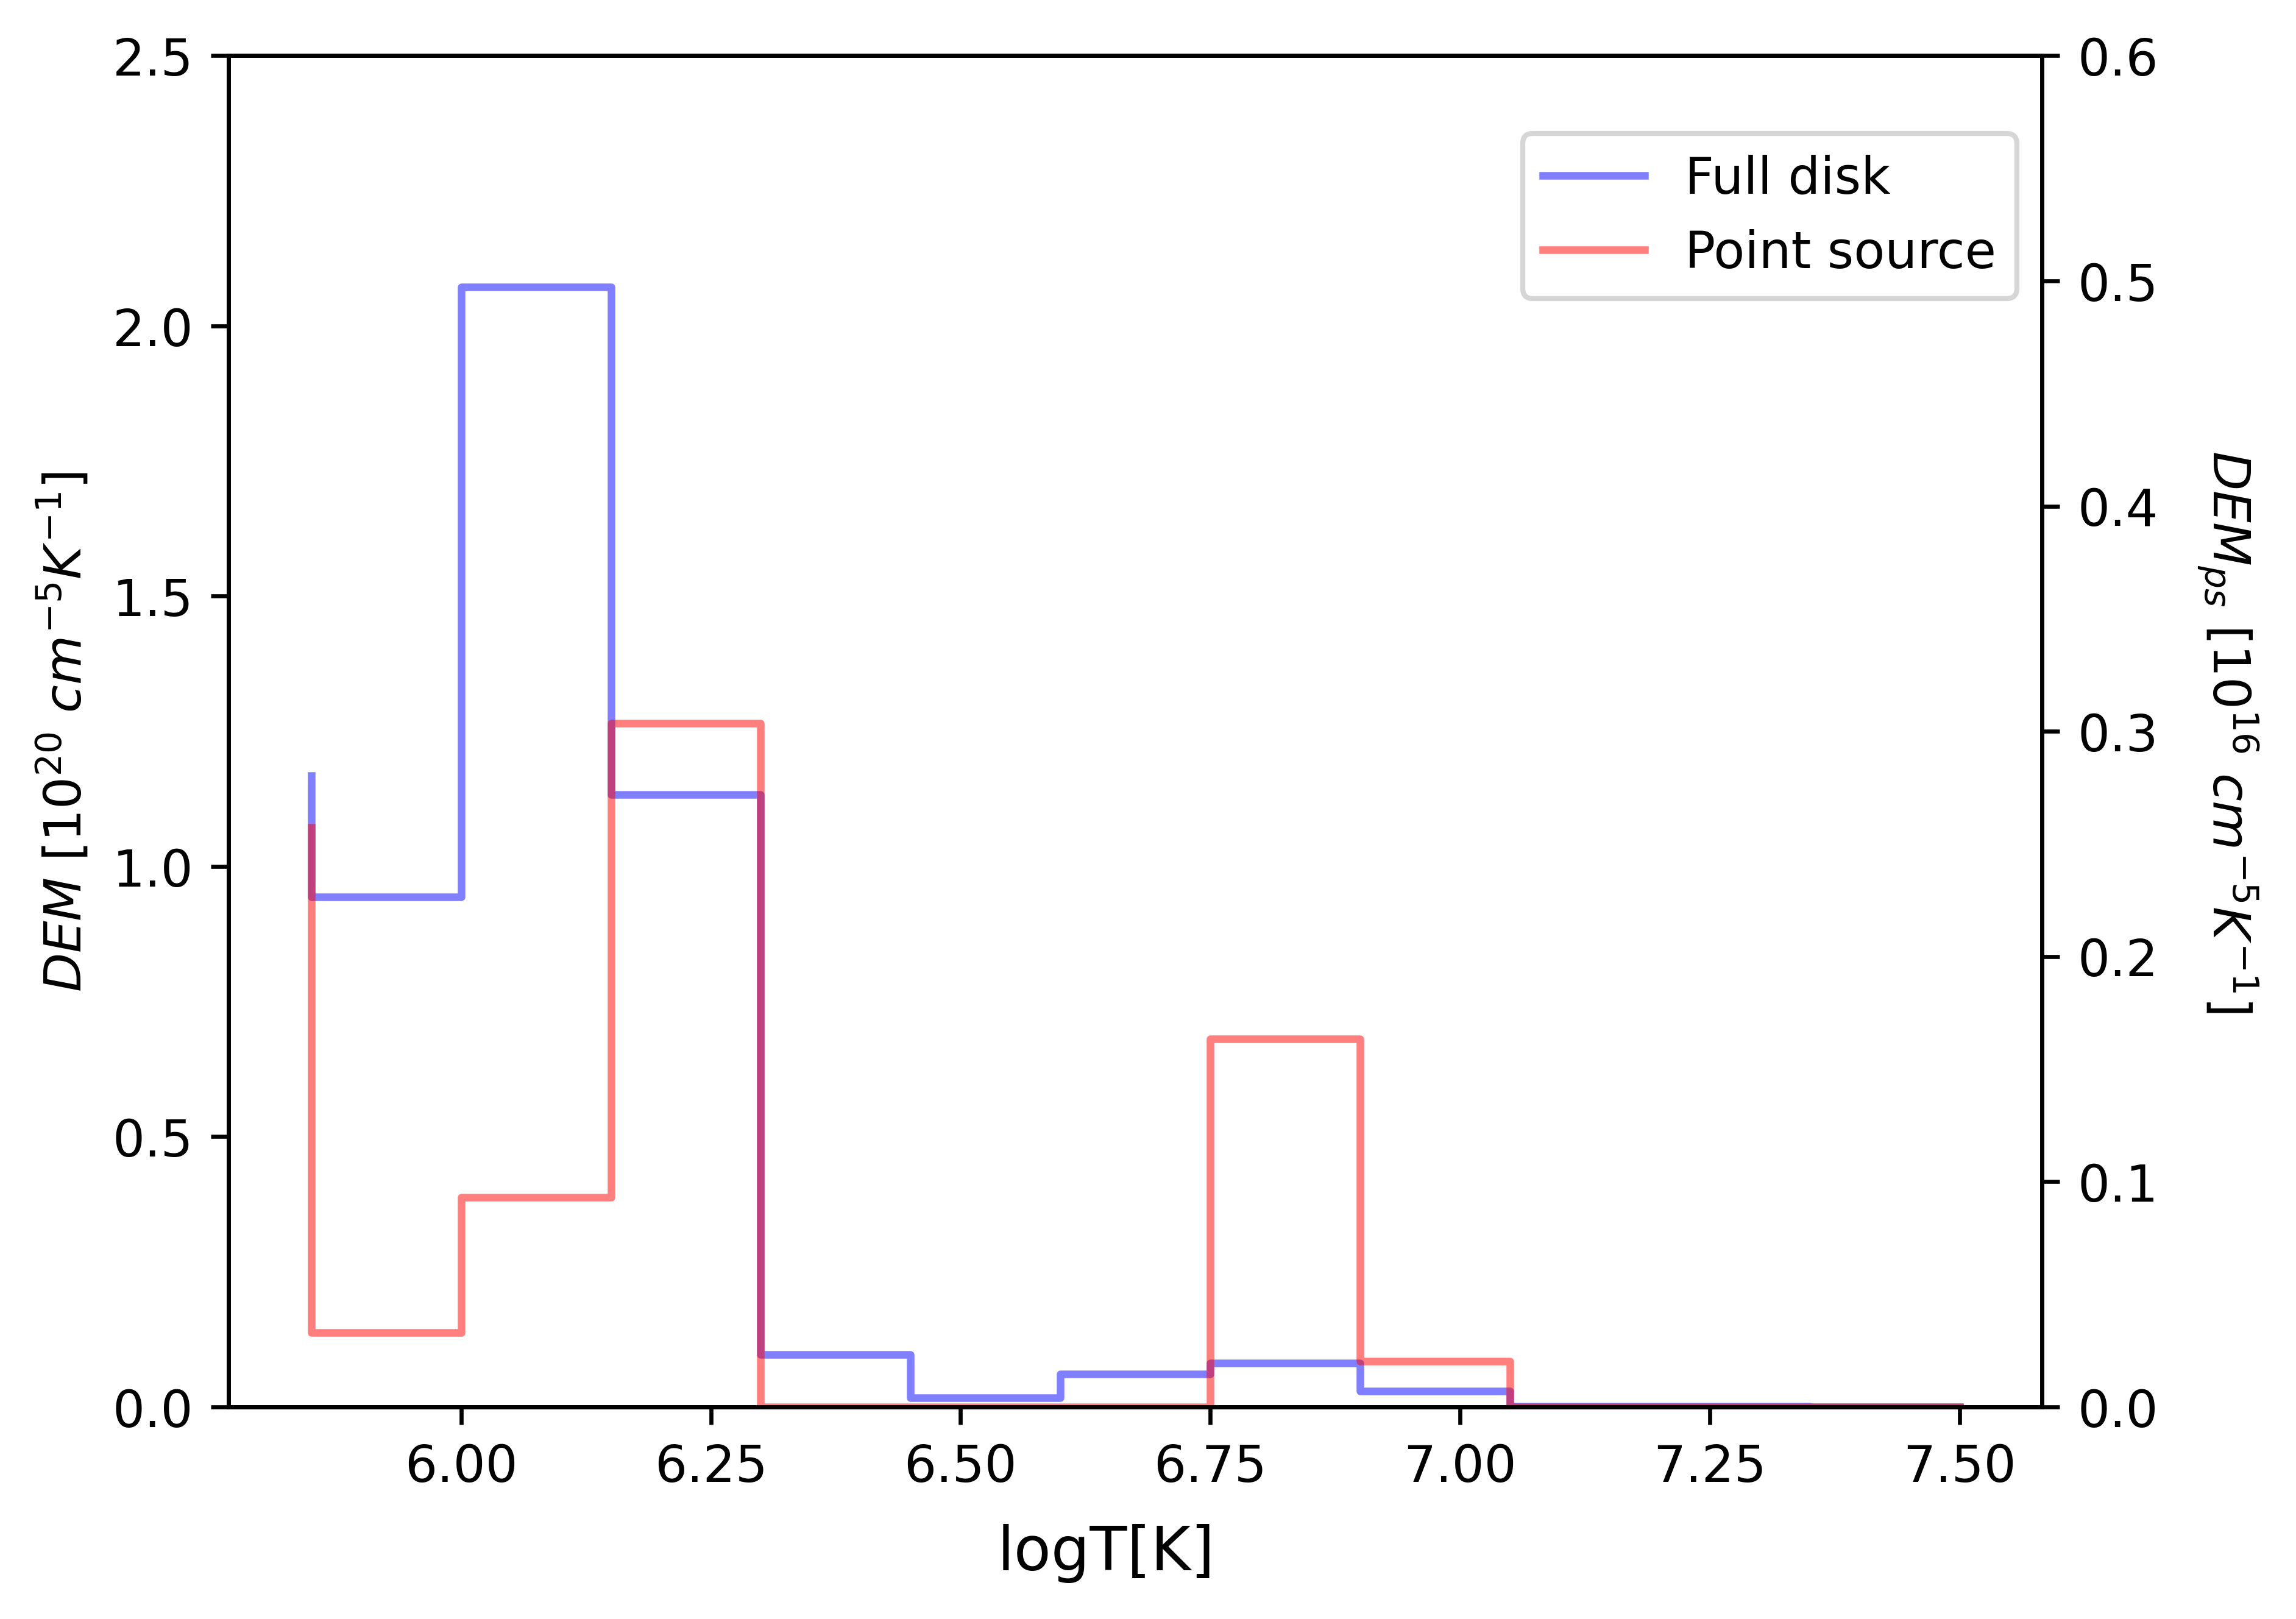
\includegraphics[width=\textwidth]{images/dem_profile_after_event_2021_oct_28.png}
        \caption{After event (17:29 UT)}
    \end{subfigure}

    \caption[DEM profile for \nth{28} October 2021 event]{DEM profile before, during and after the flaring event of \nth{28} October 2021. The red and blue curves correspond to point source and full disk source respectively}
    \label{fig:dem_pro_oct_28_2021}
\end{figure}


%%% Local Variables:
%%% mode: LaTeX
%%% TeX-master: "main"
%%% End:
